\chapter{Single Path Relay Network}
\label{chap:sp}

\begin{figure}
  \centering
    \psfrag{r0}[cc][Bl][0.9]{$r_0$}
    \psfrag{r1}[cc][Bl][0.9]{$r_1$}
    \psfrag{r3}[cc][Bl][0.9]{$r_m$}
    \psfrag{r4}[cc][Bl][0.9]{$r_{m+1}$}
    \psfrag{n0}[cc][Bl][0.8]{$n_k^{(0)}$}
    \psfrag{n2}[cc][Bl][0.8]{$n_k^{(m-1)}$}
    \psfrag{n3}[cc][Bl][0.8]{$n_k^{(m)}$}
    \psfrag{H0}[cc][Bl][0.8]{$h_k^{(0)}$}
    \psfrag{H1}[cc][Bl][0.8]{$h_k^{(1)}$}
    \psfrag{H2}[cc][Bl][0.8]{$h_k^{(m-1)}$}
    \psfrag{H3}[cc][Bl][0.8]{$h_k^{(m)}$}
    \psfrag{Tx}[cr][Bl][0.9]{Transmitter}
    \psfrag{Rx}[cl][Bl][0.9]{Receiver}
    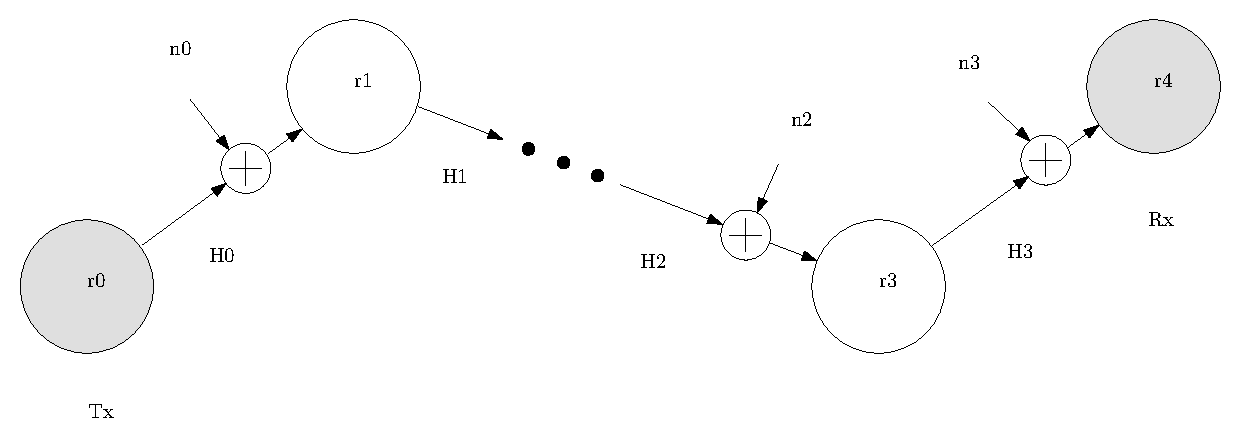
\includegraphics[width=5in]{sp_model.eps}
   \caption{Single Path Relay Network \label{fig:sp_sm} }
\end{figure}

\section{Amplify-and-Forward}
\label{sec:sp_af}

\subsection{System Model}
\label{subsec:sp_af_sm}

Figure \ref{fig:sp_sm} shows the single path relay network.  In the figure, $r_0$ is the transmitter, $r_{m+1}$ is the receiver, and $r_1, \ldots, r_m$ are $m$ relay nodes connected in series forming a single path link between the transmitter and receiver.  The relays perform amplify-and-forward (AF) relaying.  We assume that OFDM with $N$ subcarriers is used in the system.

$h_k^{(0)}, \ldots, h_k^{(m)}$ are the complex subchannel gains at the $k^{\mbox{th}}$ subcarrier in the link, for $k = 1$ to $N$.   $n_k^{(0)}, \ldots, n_k^{(m)}$ are the corresponding noises, which are assumed to be mutually independent, zero-mean, circular symmetric complex Gaussians all with variance $N_0 B / N$, where $N_0$ is the power spectral density of the underlying continuous time noise process and $B$ is the OFDM bandwidth of the system.  Let $p_k^{(0)} = P_{\mbox{tot}} / N$ be the transmitter power on the $k^{\mbox{th}}$ subcarrier, where $P_{\mbox{tot}}$ is the net transmitter power.  Let  $\sqrt{p_k^{(l)}}$ be the amplifying gain used in the amplify-and-forward algorithm at the $l^{\mbox{th}}$ relay, for $l=1$ to $m$.  The $k^{\mbox{th}}$ receive symbol at $r_l$ is amplified by $\sqrt{p_k^{(l)}}$ before it is forwarded to the next node.

Let $x_k$ be the $k^{\mbox{th}}$ transmit symbol with zero mean and unit variance.  Let $y_k$  be the $k^{\mbox{th}}$ receive symbol at the receiver.  Using Figure \ref{fig:sp_sm}, the input-output relation is


\begin{eqnarray}
y_k & = & \left( \prod_{i=0}^m h_k^{(i)} \sqrt{p_k^{(i)}}  \right) x_k + \sum_{j=0}^m 
\left( \prod_{i=j+1}^m h_k^{(i)} \sqrt{p_k^{(i)}}  \right) n_k^{(j)} \mbox{,}
\label{eqn:sp_af_inout}
\end{eqnarray}
where we assume $\prod_{i=q}^{r} a^{(i)} = 1$ for $q > r$ and any $a^{(i)}$.  We use this assumption throughout the rest of this paper.
If we define
\begin{eqnarray}
h_k = \displaystyle\prod_{i=0}^m  h_k^{(i)} \sqrt{p_k^{(i)}}
\mbox{,} & 
\gamma_k^{(j)} = \displaystyle\prod_{i=j+1}^m h_k^{(i)}  \sqrt{p_k^{(i)}}
\mbox{,}
\label{eqn:sp_af_hk_gammak}
\end{eqnarray}
\begin{eqnarray}
\mathbf{\Gamma}_k = \left[
\begin{array}{ccc}
\gamma_k^{(0)} & \cdots & \gamma_k^{(m)}
\end{array}
\right]
\mbox{,} &
\mathbf{n}_k = \left[
\begin{array}{ccc}
n_k^{(0)} & \cdots & n_k^{(m)}
\end{array} \right]^T\mbox{,}
\label{eqn:sp_af_Gammak_nk}
\end{eqnarray}
and
\begin{eqnarray}
w_k = \mathbf{\Gamma}_k \mathbf{n}_k \mbox{,} 
\label{eqn:sp_af_wk}
\end{eqnarray}
then (\ref{eqn:sp_af_inout}) can be written as
\begin{eqnarray}
y_k = h_k x_k + w_k \mbox{.}
\label{eqn:sp_af_inout_terse}
\end{eqnarray}

Now, consider the variance of $w_k$.  Using (\ref{eqn:sp_af_hk_gammak}), (\ref{eqn:sp_af_Gammak_nk}), and (\ref{eqn:sp_af_wk}), we have
\begin{eqnarray}
R_{w_kw_k} & = & E \left[ w_k w_k^* \right] \\
& = & E \left[ \mathbf{\Gamma}_k \mathbf{n}_k \mathbf{n}_k^H \mathbf{\Gamma}_k^H \right] \\
& = & \mathbf{\Gamma}_k E \left[ \mathbf{n}_k \mathbf{n}_k^H  \right] \mathbf{\Gamma}_k^H \\
    & = & \frac{N_0B}{N} \sum_{j=0}^{m} \left( \prod_{i=j+1}^mb_k^{(i)}  p_k^{(i)}  \right) ,
\label{eqn:sp_af_Rwkwk}
\end{eqnarray}
where $E\left[ \cdot \right]$ is the expectation operator, $\left(\cdot\right)^*$ is the complex conjugate operator for a scalar, $\left( \cdot \right)^H$ is the Hermitian (complex transpose) operator for a vector or matrix, and $b_k^{(i)} = \left| h_k^{(i)} \right|^2$, for $i=0$ to $m$.  $R_{w_kw_k}$ is positive for a nonzero $N_0$.  We define a transformed version of the system in (\ref{eqn:sp_af_inout_terse})
\begin{eqnarray}
\tilde{y}_k = \tilde{h}_k x_k + \tilde{w}_k,
\end{eqnarray}
where $\tilde{y}_k = y_k / \sqrt{R_{w_kw_k}}$, $\tilde{h}_k = h_k / \sqrt{R_{w_kw_k}}$, and $\tilde{w}_k = w_k / \sqrt{R_{w_kw_k}}$.  The variances of $\tilde{w}_k$ and $\tilde{y}_k$ are
\begin{eqnarray}
E \left[ \tilde{w}_k \tilde{w}_k^* \right] & = & E \left[ \frac{w_k}{\sqrt{R_{w_kw_k}}} \frac{w_k^*}{\sqrt{R_{w_kw_k}}} \right] \\
& = & \frac{R_{w_kw_k}}{R_{w_kw_k}} \\
& = & 1
\end{eqnarray}
and
\begin{eqnarray}
E \left[ \tilde{y}_k \tilde{y}_k^* \right] & = & E \left[ \left( \tilde{h}_k x_k + \tilde{w}_k \right) \left( \tilde{h}_k x_k + \tilde{w}_k \right)^* \right] \\
& = & \tilde{h}_k \tilde{h}_k^* + 1 \\
& = & \frac{1}{R_{w_kw_k}} \left( \prod_{i=0}^m b_k^{(i)} p_k^{(i)} \right) + 1
\label{eqn:sp_af_yk_tilde_var} \mbox{,}
\end{eqnarray}
respectively.  The cross terms do not appear in (\ref{eqn:sp_af_yk_tilde_var}) because $\tilde{h_k}$, $\tilde{w_k}$, and $x_k$ are mutually independent.  Note that the transformed system has unit variance noise.

\subsection{Mutual Information}
\label{subsec:sp_af_mi}

To derive the mutual information, note that the differential entropy of a circular symmetric complex Gaussian vector, $\mathbf{v}$, with covariance matrix, $\mathbf{K}$, is $h\left(\mathbf{v}\right) = \log_2 \det \left( \pi e \mathbf{K} \right)$ \cite{article:Telatar01}.  When the circular symmetric complex Gaussian is a scalar, $v$, the differential entropy is $h\left(v\right) = \log_2 \left( \pi e \sigma_v^2 \right)$, where $\sigma_v^2$ is the variance of $v$.  Let $\mathcal{I}_k$ be the mutual information between the transmitter and receiver on the $k^{\mbox{th}}$ subcarrier
\begin{eqnarray}
\mathcal{I}_k & = & h\left( \tilde{y}_k \right) - h \left( \tilde{w}_k \right) \\
& = & \log_2 \left( \pi e \left[ \frac{1}{R_{w_kw_k}} \left( \prod_{i=0}^m b_k^{(i)} p_k^{(i)} \right) + 1 \right] \right)
- \log_2 \left( \pi e \right) \\
& = & \log_2 \left[ \frac{1}{R_{w_kw_k}} \left( \prod_{i=0}^m b_k^{(i)} p_k^{(i)} \right) + 1 \right],
\label{eqn:sp_af_Ik}
\end{eqnarray}
where the first equality comes from basic mutual information calculations \cite{book:Cover01}.  The total mutual information between the transmitter and receiver, $\mathcal{I}$, is the sum of all $\mathcal{I}_k$ divided by $N$.  That is, after substituting (\ref{eqn:sp_af_Rwkwk}) into (\ref{eqn:sp_af_Ik}), we have
\begin{eqnarray}
\mathcal{I} & = &\frac{1}{N} \sum_{k=1}^N \mathcal{I}_k\\
& = &\frac{1}{N} \sum_{k=1}^N \log_2 \left( 1 + \mbox{SNR}
\left[ \frac{b_k^{(0)}\left( \prod_{i=1}^m b_k^{(i)}  p_k^{(i)}  \right)}
{\sum_{j=0}^m \left( \prod_{i=j+1}^m b_k^{(i)}  p_k^{(i)}  \right) }\right]
 \right),
\label{eqn:sp_af_I}
\end{eqnarray}
where $\mbox{SNR} = P_{\mbox{tot}} / N_0 B$.  If we denote
\begin{eqnarray}
\begin{array}{ccc}
\mathbf{b}^{(i)} = \left[ \begin{array}{ccc}
b_1^{(i)} & \cdots & b_N^{(i)}
\end{array}
\right]^T &  \mbox{and} &   
\mathbf{p}^{(i)} = \left[ \begin{array}{ccc}
p_1^{(i)} & \cdots & p_N^{(i)}
\end{array}
\right]^T,
\end{array} 
\end{eqnarray} 
for $i = 0$ to $m$ and
\begin{eqnarray}
\mathbf{e}_N = \underbrace{ \left[ \begin{array}{ccc}
1 & \cdots & 1
\end{array}
\right]^T}_{\mbox{$N$ ones}},
\end{eqnarray}
then (\ref{eqn:sp_af_I}) can be written in matrix form.  First, let
\begin{eqnarray}
\mathbf{z}_{\mbox{single}} = \left[ \mathbf{b}^{(0)} \circ \left( \circ \prod_{i=1}^m \mathbf{b}^{(i)} \circ  \mathbf{p}^{(i)}  \right) \right] \circ / 
\left[ \sum_{j=0}^{m} \left(\circ \prod_{i=j+1}^{m}  \mathbf{b}^{(i)} \circ \mathbf{p}^{(i)} \right) \right],
\end{eqnarray}
where the $\circ$ and $\circ \prod$ operators both represent element-wise matrix multiplication and the $\circ /$ operator represents element-wise matrix division.  Then, (\ref{eqn:sp_af_I}) in matrix form is
\begin{eqnarray}
\mathcal{I} = \frac{1}{N}\mathbf{e}_N^T  \log_2 \left( \mathbf{e}_N + \mbox{SNR} \: \mathbf{z}_{\mbox{single}} \right),
\label{eqn:sp_af_I_matrix}
\end{eqnarray}
where $\log_2\left( \cdot \right)$ of a vector is the vector of the logarithms of the vector's entries.

\subsection{Relay Power Allocation}
\label{subsec:sp_af_rpa}

We assume that the net transmit power at the transmitter and at each each relay is $P_{\mbox{tot}}$.  At the transmitter, we assume a uniform power distribution, that is, $p_k^{(0)} = P_{\mbox{tot}}/N$.  To derive the power constraint at each relay and thus, possible power allocations, consider $v_k^{(l)}$, the $k^{\mbox{th}}$ transmit symbol of $r_l$
\begin{eqnarray}
v_k^{(l)} = \sqrt{p_k^{(l)}} \left[ \left( \prod_{i=0}^{l-1} h_k^{(i)}  \sqrt{p_k^{(i)}} \right)  x_k + \sum_{j=0}^{l-1}\left( \prod_{i=j+1}^{l-1} h_k^{(i)}  \sqrt{p_k^{(i)}} \right)n_k^{(j)} \right] \mbox{.}
\end{eqnarray}
The constraint is $P_{\mbox{tot}} = \displaystyle \sum_{k=1}^{N} E \left[ \left| v_k^{(l)} \right|^2 \right]$.  Thus,
\begin{eqnarray}
P_{\mbox{tot}} = \displaystyle \sum_{k=1}^{N} p_k^{(l)}
\left[ b_k^{(0)} \frac{P_{\mbox{tot}}}{N}  \left( \displaystyle \prod_{i=1}^{l-1}  b_k^{(i)} p_k^{(i)} \right) + 
\frac{N_0 B}{N} \sum_{j=0}^{l-1} \left( \displaystyle \prod_{i=j+1}^{l-1}  b_k^{(i)} p_k^{(i)} \right) 
\right]
\label{eqn:sp_af_powerconstraint0}
\end{eqnarray}
or
\begin{eqnarray}
\sum_{k=1}^N \frac{ p_k^{(l)}}{N} \left[
b_k^{(0)} \left( \prod_{i=1}^{l-1}  b_k^{(i)}p_k^{(i)} \right) + 
\frac{1}{\mbox{SNR}} \sum_{j=0}^{l-1} \left( \prod_{i=j+1}^{l-1}  b_k^{(i)}p_k^{(i)}
\right)
\right] =1.
\label{eqn:sp_af_powerconstraint}
\end{eqnarray}
Note that (\ref{eqn:sp_af_powerconstraint}) is defined recursively.  The power constraint for $p_k^{(l)}$ depends on $p_k^{(1)}, \dots, p_k^{(l-1)}$.  $p_k^{(1)}$ is the base case in the recursion, which follows from (\ref{eqn:sp_af_powerconstraint}), when $l = 1$.

One power allocation at the $l^{\mbox{th}}$ relay is to set $p_k^{(l)}$ constant for all subcarriers.  This results in moving $p_k^{(l)}$ in (\ref{eqn:sp_af_powerconstraint}) out of the summation because it is no longer a function of $k$
\begin{eqnarray}
p_{k,ct}^{(l)} = p_{ct}^{(l)} = 
 \frac{N \mbox{SNR}}
{\displaystyle \sum_{k=1}^N \left[ \mbox{SNR} b_k^{(0)} \left( \displaystyle \prod_{i=1}^{l-1} b_k^{(i)} p_{ct}^{(i)}\right) + \displaystyle \sum_{j=0}^{l-1} \left( \displaystyle \prod_{i=j+1}^{l-1} b_k^{(i)} p_{ct}^{(i)}\right)
\right]
} \mbox{.}
\end{eqnarray}
We call this \emph{constant gain allocation} (CT).  Note that this power allocation does not require each relay to have any CSI (channel state information).  The $l^{\mbox{th}}$ relay only has to multiply its entire OFDM receive symbol by a constant, $\sqrt{p_{ct}^{(l)}}$, such that the total transmit power is $P_{\mbox{tot}}$.  We call \emph{constant gain capacity}, $C_{ct}$, as the mutual information in (\ref{eqn:sp_af_I_matrix}) resulting from this power allocation.

A second power allocation is to choose $p_k^{(l)}$ such that every subcarrier transmits the same power at the $l^{\mbox{th}}$ relay.  The transmit power on the $k^{\mbox{th}}$ subcarrier is the $k^{\mbox{th}}$ summand on the right hand side of (\ref{eqn:sp_af_powerconstraint0}).  Since they are all equal to $P_{\mbox{tot}}/N$, we have
\begin{eqnarray}
\frac{P_{\mbox{tot}}}{N} = 
 p_{k,eq}^{(l)}
\left[b_k^{(0)} \frac{P_{\mbox{tot}}}{N}  \left( \displaystyle \prod_{i=1}^{l-1} b_k^{(i)} p_{k,eq}^{(i)} \right) + 
\frac{N_0 B}{N} \sum_{j=0}^{l-1} \left( \displaystyle \prod_{i=j+1}^{l-1} b_k^{(i)} p_{k,eq}^{(i)} \right) 
\right]\end{eqnarray}
or
\begin{eqnarray}
p_{k,eq}^{(l)} = \frac{\mbox{SNR}}
{\mbox{SNR} b_k^{(0)} \left( \displaystyle\prod_{i=1}^{l-1}b_k^{(i)} p_{k,eq}^{(i)} \right) + \displaystyle\sum_{j=0}^{l-1} \left(
\prod_{i=j+1}^{l-1}  b_k^{(i)} p_{k,eq}^{(i)}
\right)} \mbox{.}
\label{}
\end{eqnarray}
We call this \emph{equal power allocation} (EQ).  Note that this power allocation does require each relay to have the CSI of its upstream channels.  We call \emph{equal power capacity}, $C_{eq}$, as the mutual information in (\ref{eqn:sp_af_I_matrix}) resulting from this power allocation.

\subsection{Capacity Simulations}
\label{subsec:sp_af_cs}

We simulate $C_{ct}$ and $C_{eq}$ assuming that all distances between any two adjacent transceiver nodes are the same.  Therefore, all path loss effects are normalized to $0$ dB.  Shadowing between nodes is assumed to be log-normally distributed.  That is, the received power gain due to shadowing in dB is a zero-mean Gaussian with variance of 8 dB, which is typical for cellular land mobile applications \cite{book:Stuber01}.  We model frequency selective fading effects as Typical Urban (TU) channels and Hilly Terrain (HT) channels \cite{book:Stuber01}.  We use an OFDM bandwidth of 800 kHz divided into $N=128$ equal blocks.  Maintaining OFDM orthogonality, this translates into an OFDM symbol period of $T_s = 160\:\mu$s.  Results are shown in Figures \ref{fig:sp_af_cap_plots_TU} and  \ref{fig:sp_af_cap_plots_HT}.

The plots exhibit the familiar monotonically increasing shape for mutual information in the case of direct transmission between a transmitter and receiver.  This is expected if we look at the mutual information in (\ref{eqn:sp_af_I_matrix}).  We can think of this configuration as still being direct transmission where the channel is the single path relay network, characterized by $\mathbf{z}_{\mbox{single}}$.  Note that $\mathbf{z}_{\mbox{single}}$ also determines the power allocations in the relays.  In other words, (\ref{eqn:sp_af_I_matrix}) is a system level representation of the mutual information.

As we increase the distance between the transmitter and receiver (and thus, add more relays), more noise and channel distortion enter the system.  Consequently, the mutual information decreases.  Equal power allocation results in a slightly higher mutual information than that of constant gain allocation.  TU channels and HT channels give very similar results.

\begin{figure*}
    \psfrag{Capacity}[Bc][tc][0.8]{Capacity (bits/s/Hz)}
    \psfrag{SNR}[tc][Bc][0.8]{SNR (dB)}
    \psfrag{Cct-}[cl][cl][0.6]{$C_{ct}$}
    \psfrag{Ceq-}[cl][cl][0.6]{$C_{eq}$}
    \psfrag{Caa-}[cl][cl][0.6]{$C_{aa}$}
\centerline{
	\subfigure[m=1]{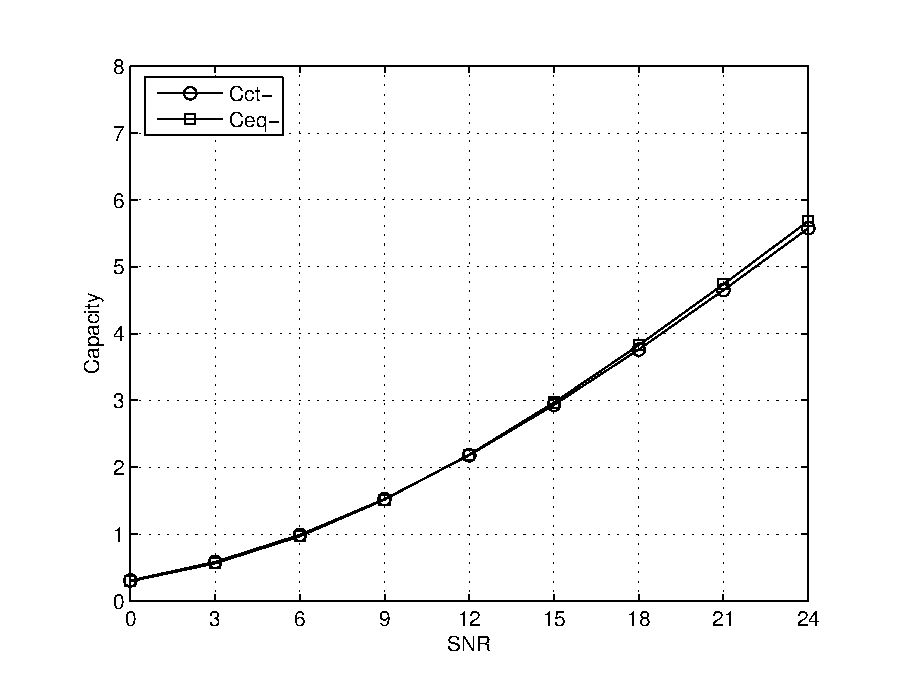
\includegraphics[width=3in]{sp_af_cap_m1_TU.eps} \label{}} 
	\subfigure[m=2]{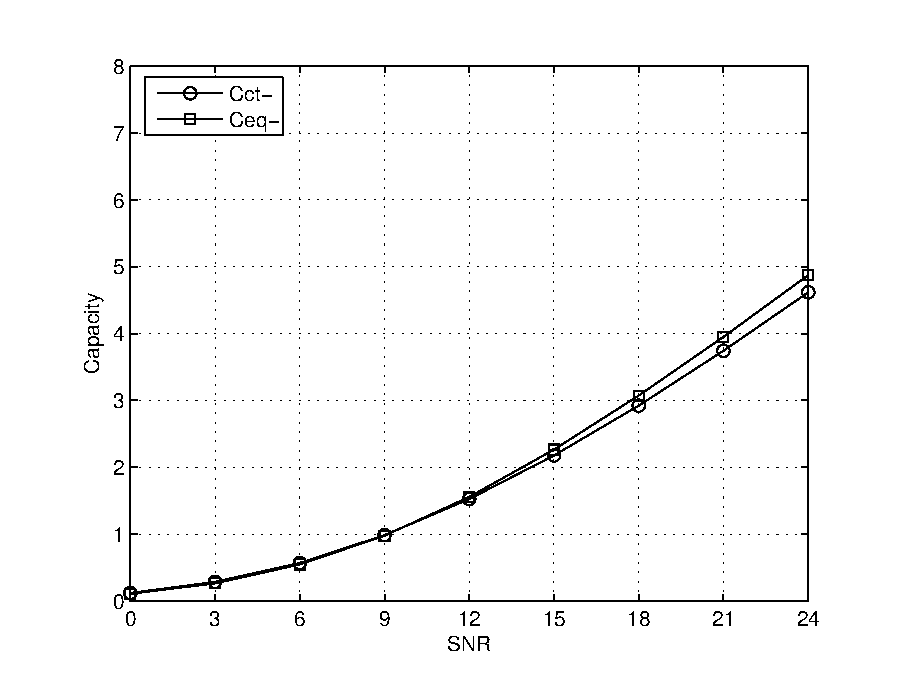
\includegraphics[width=3in]{sp_af_cap_m2_TU.eps} \label{}} \\
}
\centerline{
	\subfigure[m=3]{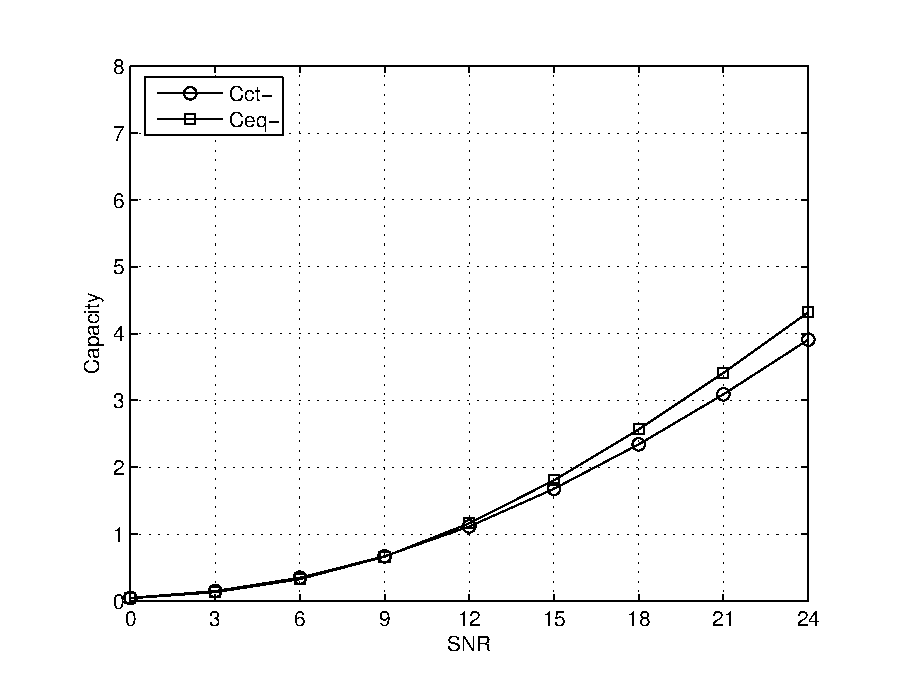
\includegraphics[width=3in]{sp_af_cap_m3_TU.eps} \label{}}
	\subfigure[m=4]{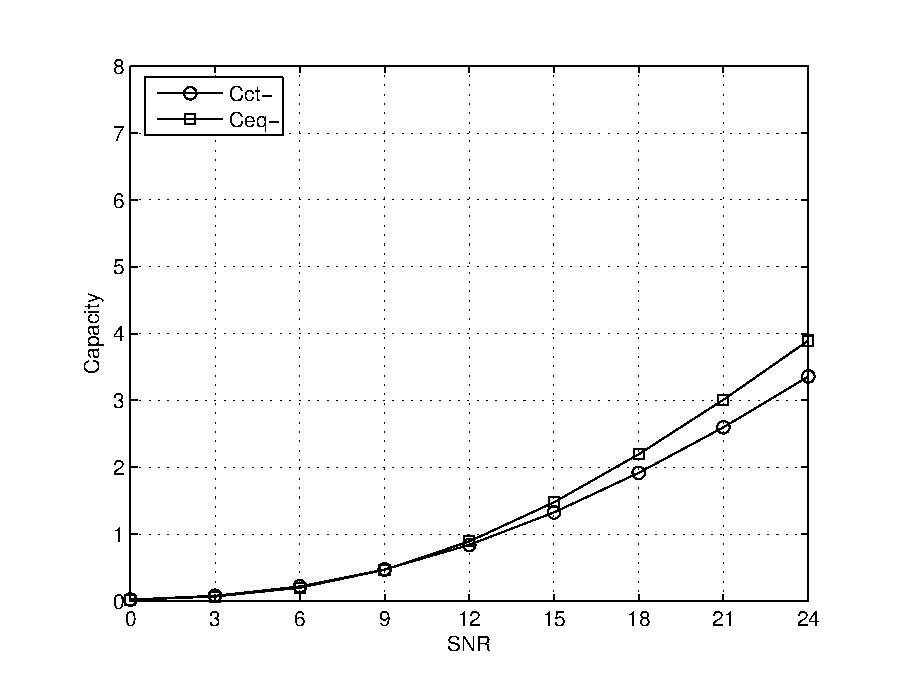
\includegraphics[width=3in]{sp_af_cap_m4_TU.eps} \label{}} \\
}
\caption{Capacity in a single path relay network with TU channels using AF.  $N = 128, m = 1, 2, 3$, and $4$.}
\label{fig:sp_af_cap_plots_TU}
\end{figure*}

\begin{figure*}
    \psfrag{Capacity}[Bc][tc][0.8]{Capacity (bits/s/Hz)}
    \psfrag{SNR}[tc][Bc][0.8]{SNR (dB)}
    \psfrag{Cct-}[cl][cl][0.6]{$C_{ct}$}
    \psfrag{Ceq-}[cl][cl][0.6]{$C_{eq}$}
    \psfrag{Caa-}[cl][cl][0.6]{$C_{aa}$}
\centerline{
	\subfigure[m=1]{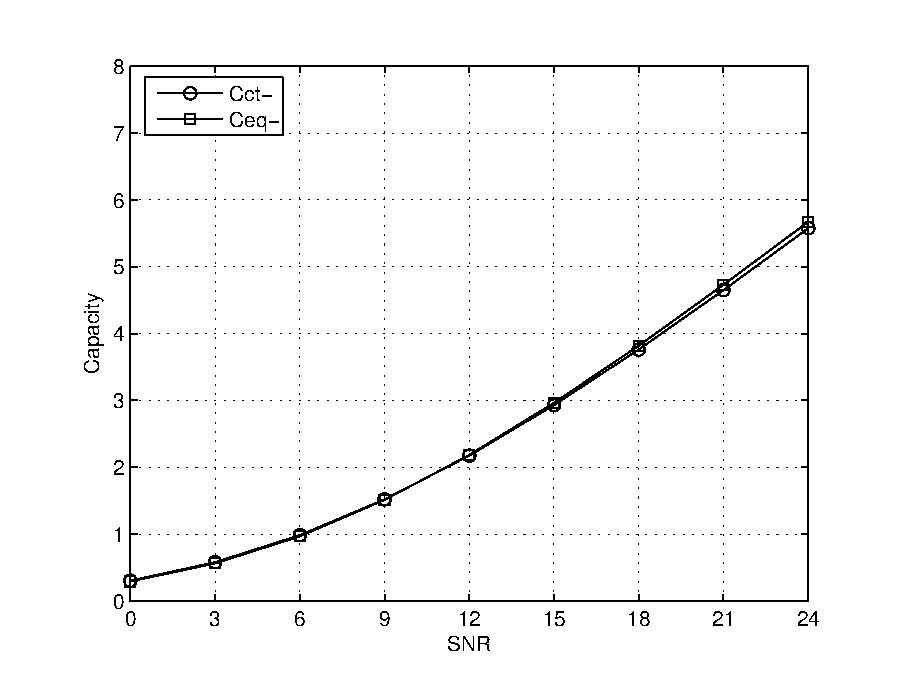
\includegraphics[width=3in]{sp_af_cap_m1_HT.eps} \label{}} 
	\subfigure[m=2]{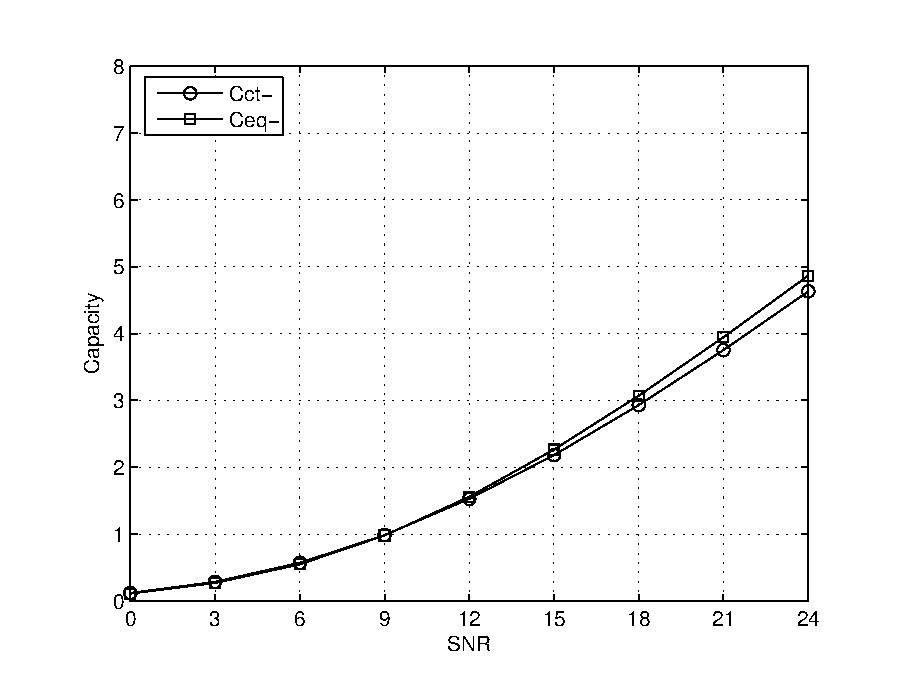
\includegraphics[width=3in]{sp_af_cap_m2_HT.eps} \label{}} \\
}
\centerline{
	\subfigure[m=3]{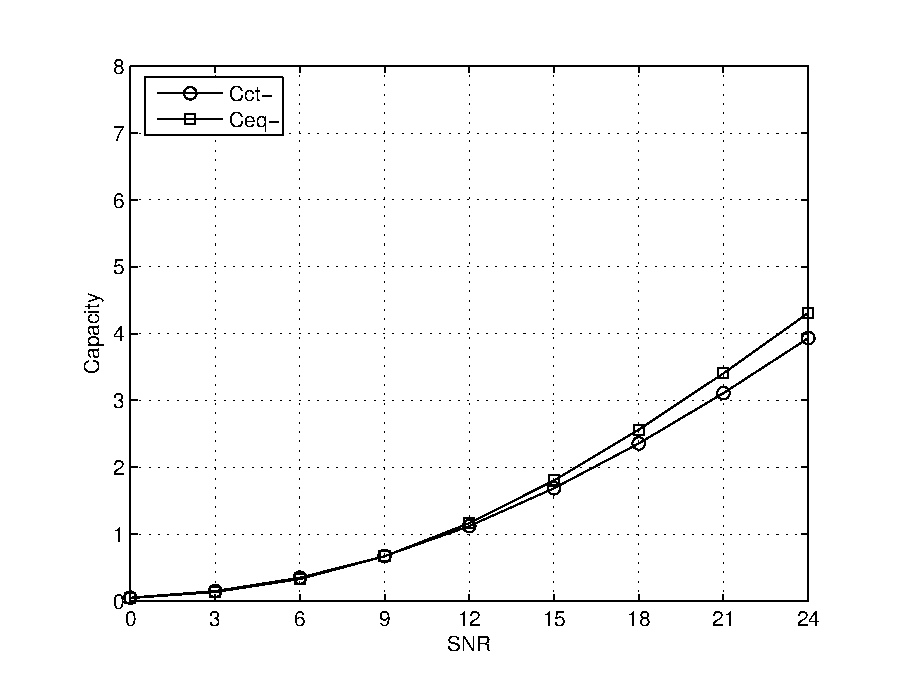
\includegraphics[width=3in]{sp_af_cap_m3_HT.eps} \label{}}
	\subfigure[m=4]{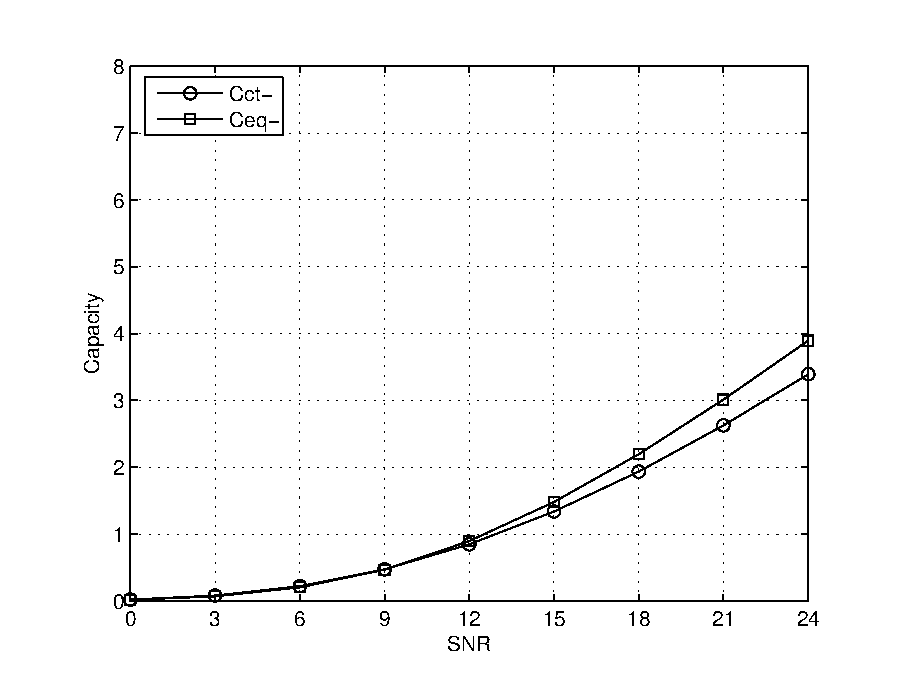
\includegraphics[width=3in]{sp_af_cap_m4_HT.eps} \label{}} \\
}
\caption{Capacity in a single path relay network with HT channels using AF.  $N = 128, m = 1, 2, 3$, and $4$.}
\label{fig:sp_af_cap_plots_HT}
\end{figure*}


\section{Decode-and-Forward}
\label{sec:sp_df}

\subsection{System Model}
\label{subsec:sp_df_sm}

In decode-and-forward (DF), each relay fully recovers the information bits (with possible errors) after receiving an OFDM symbol.  It then converts the information bits back into an OFDM symbol and then transmits it.  The transmitter and all the relays transmit with the same uniform power distribution.  That is,
\begin{eqnarray}
p_k^{(0)} = p_k^{(l)} = \frac{P_{\mbox{tot}}}{N}\mbox{,}
\end{eqnarray}
for $k = 1$ to $N$ and for $l = 1$ to $m$.

Let $x_k^{(0)}$ be the $k^{\mbox{th}}$ transmit symbol from the transmitter and  $x_k^{(l)}$ be the $k^{\mbox{th}}$ transmit symbol from the $l^{\mbox{th}}$ relay, all with with zero mean and unit variance.  Let $y_k^{(m+1)}$ be the $k^{\mbox{th}}$ receive symbol at the receiver and  $y_k^{(l)}$ be the $k^{\mbox{th}}$ receive symbol at the $l^{\mbox{th}}$ relay.  Using Figure \ref{fig:sp_sm}, the input-ouput relation at the $l^{\mbox{th}}$ relay is
\begin{eqnarray}
y_k^{(l)} = h_k^{(l-1)} \sqrt{\frac{P_{\mbox{tot}}}{N}} x_k^{(l-1)} + n_k^{(l-1)} \mbox{.}
\end{eqnarray}
The input-output relation at the receiver is
\begin{eqnarray}
y_k^{(m+1)} =h_k^{(m)}  \sqrt{\frac{P_{\mbox{tot}}}{N}} x_k^{(m)} + n_k^{(m)} \mbox{.}
\end{eqnarray}

\section{BER and WER Simulations}
\label{sec:sp_bws}

\begin{figure}
  \centering
    \psfrag{in}[cr][cc][0.9]{input}
    \psfrag{o1}[cl][Bl][0.9]{output 1}
    \psfrag{o2}[cl][Bl][0.9]{output 2}
    \psfrag{o3}[cl][Bl][0.9]{output 3}
    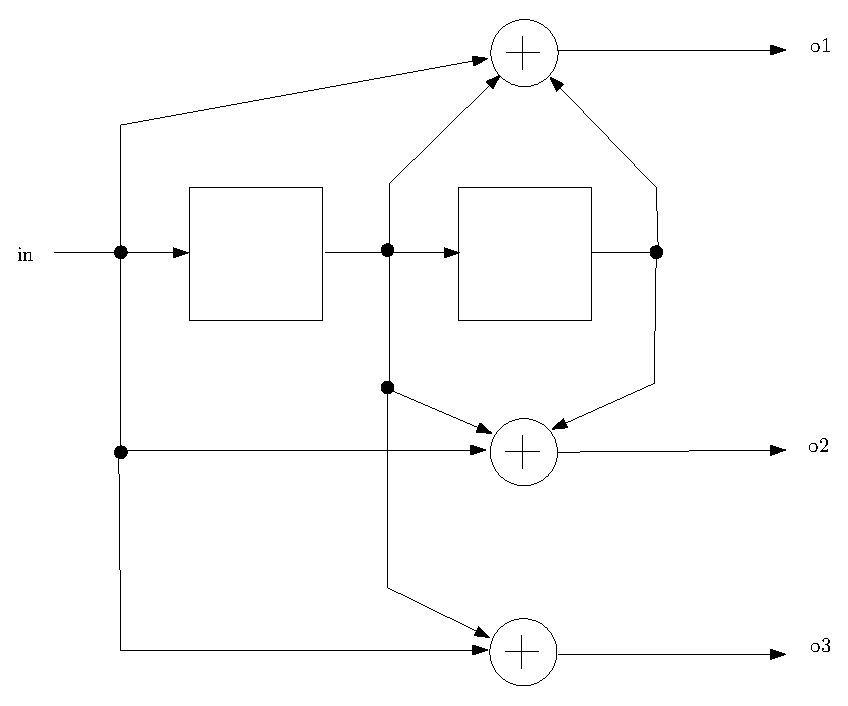
\includegraphics[width=4in]{conv_enc.eps}
   \caption{Convolutional encoder. \label{fig:conv_enc} }
\end{figure}

We simulate bit error rates (BERs) and word error rates (WERs) for both the amplify-and-forward and decode-and-forward cases.  At the transmitter (and at the transmitter structure of a relay using decode-and-forward), each information word contains 83 bits.  Using the convolutional encoder shown in Figure \ref{fig:conv_enc}, the information word is encoded into a 255 bit codeword.  A zero bit is padded at the end to make 256 bits.  The bits are then interleaved and modulated onto $N = 128$ QPSK (quadrature phase shift keying) subcarriers to form one OFDM symbol.  At the receiver (and at the receiver structure of a relay using decode-and-forward), the codeword is recovered (with possible errors) using a matched filter and deinterleaving.  A Viterbi decoder is used to decode the codeword.  Both hard decisions and soft decisions are used.

We assume that all distances between any two adjacent transceiver nodes are the same.  Therefore, all path loss effects are normalized to 0 dB.  Shadowing is assumed to be log-normally distributed.  That is, the received power gain due to shadowing in dB is a zero-mean Gaussian with variance of 8 dB, which is typical for cellular land mobile applications \cite{book:Stuber01}.  We model frequency selective fading as Typical Urban (TU) channels and Hilly Terrain (HT) channels \cite{book:Stuber01}.  We use an OFDM bandwidth of 800 kHz divided into $N = 128$ equal blocks.  Maintaining OFDM orthogonality, this translates into an OFDM symbol period of $T_s = 160 \:\mu$s.  

\subsection{Amplify-and-Forward}
\label{subsec:sp_bws_af}

The BER versus SNR and WER versus SNR plots for a single path relay network with TU channels using amplify-and-forward are shown in Figures \ref{fig:sp_af_ber_plots_TU} and \ref{fig:sp_af_wer_plots_TU}, respectively.  The corresponding plots for HT channels are shown in Figures \ref{fig:sp_af_ber_plots_HT} and \ref{fig:sp_af_wer_plots_HT}, respectively.

As expected, soft decisions in Viterbi decoding give better performance than hard decisions.  In particular, there is up to 4 dB of SNR gain for the constant gain allocation and $m=1$ case, as shown in Figures \ref{fig:sp_af_ber_m1_TU}, \ref{fig:sp_af_wer_m1_TU}, \ref{fig:sp_af_ber_m1_HT}, and \ref{fig:sp_af_wer_m1_HT}.  In general, using hard decisions with constant gain allocation results in the worst performance.  Soft decisions with equal power allocation gives the best performance, except for the $m=1$ case, where soft decisions with constant gain allocation is slightly better.  

As we increase the distance between the transmitter and receiver (and thus, add more relays), more noise and channel distortion enter the system.  Consequently, the error rate (BER and WER) performance becomes worse and as a result, all four curves are very close together at low to medium SNR values.  TU channels and HT channels give very similar results.

\begin{figure*}
    \psfrag{BER}[Bc][tc][0.8]{BER}
    \psfrag{SNR}[tc][Bc][0.8]{SNR (dB)}
    \psfrag{hard--constant-gain-allocation}[cl][cl][0.5]{hard, constant gain allocation}
    \psfrag{hard--equal-power-allocation}[cl][cl][0.5]{hard, equal power allocation}
    \psfrag{soft--constant-gain-allocation}[cl][cl][0.5]{soft, constant gain allocation}
    \psfrag{soft--equal-power-allocation}[cl][cl][0.5]{soft, equal power allocation}

\centerline{
	\subfigure[m=1]{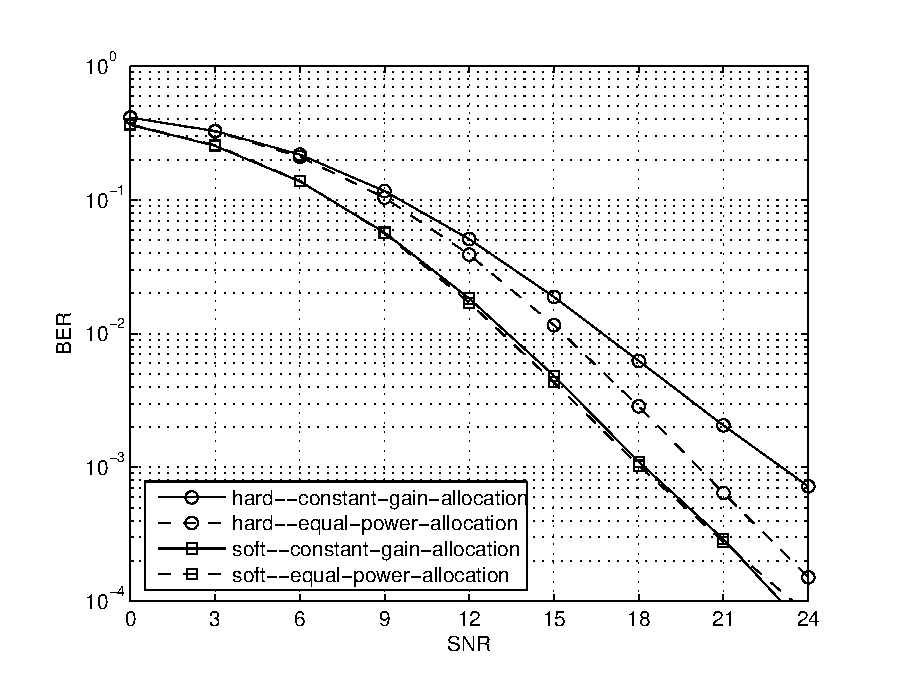
\includegraphics[width=3in]{sp_af_ber_m1_TU.eps} \label{fig:sp_af_ber_m1_TU}} 
	\subfigure[m=2]{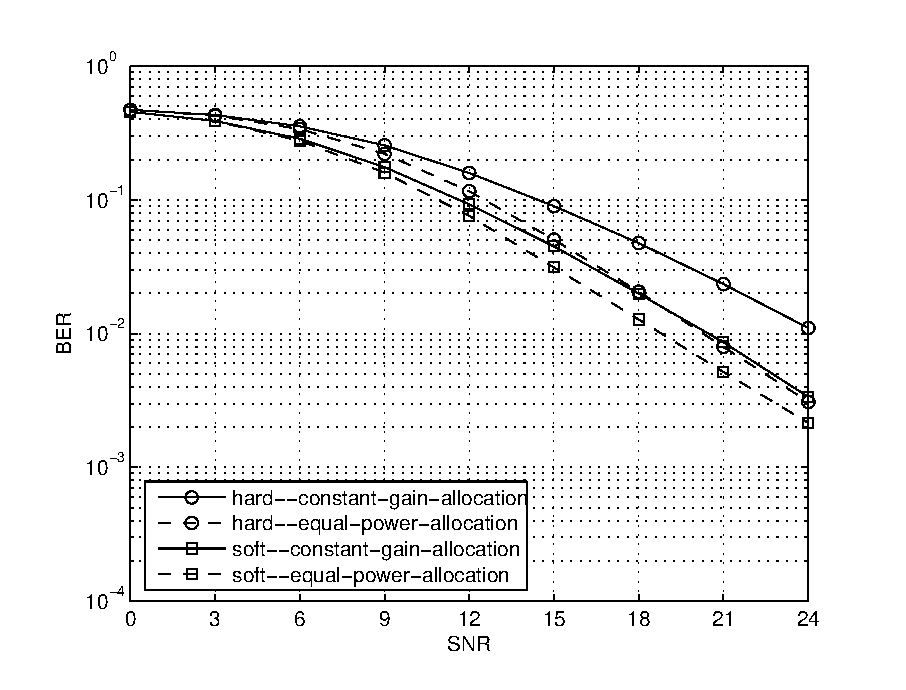
\includegraphics[width=3in]{sp_af_ber_m2_TU.eps} \label{}} \\
}
\centerline{
	\subfigure[m=3]{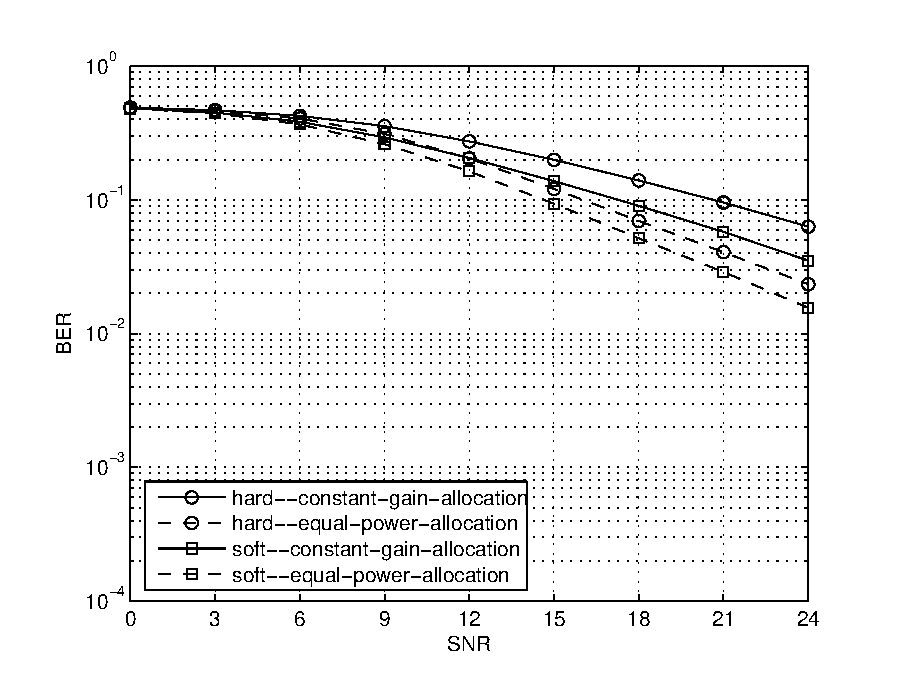
\includegraphics[width=3in]{sp_af_ber_m3_TU.eps} \label{}}
	\subfigure[m=4]{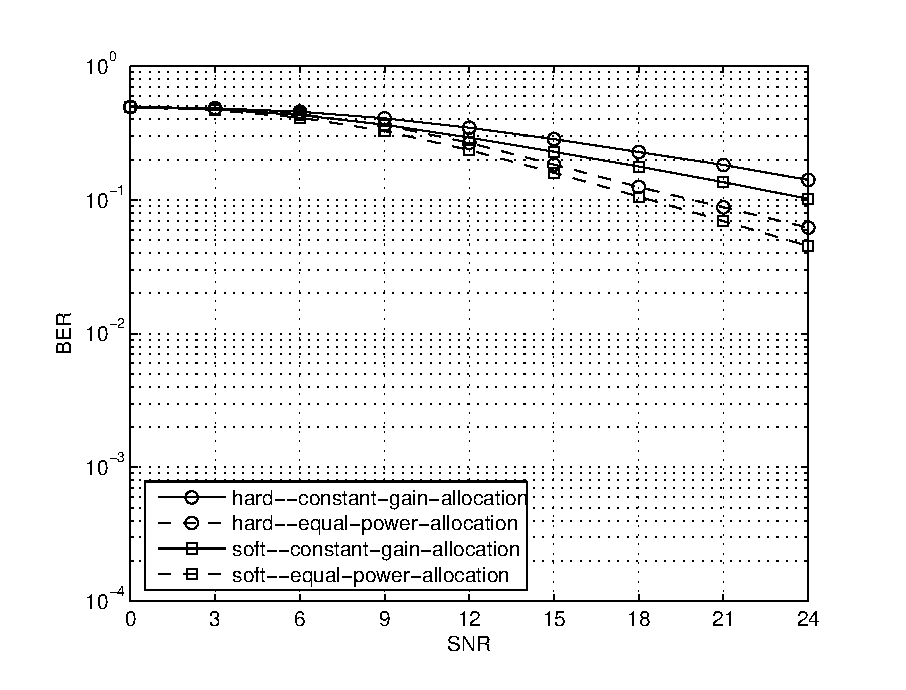
\includegraphics[width=3in]{sp_af_ber_m4_TU.eps} \label{}} \\
}
\caption{BER in a single path relay network with TU channels using AF.  $N = 128, m = 1, 2, 3$, and $4$.}
\label{fig:sp_af_ber_plots_TU}
\end{figure*}

\begin{figure*}
    \psfrag{WER}[Bc][tc][0.8]{WER}
    \psfrag{SNR}[tc][Bc][0.8]{SNR (dB)}
    \psfrag{hard--constant-gain-allocation}[cl][cl][0.5]{hard, constant gain allocation}
    \psfrag{hard--equal-power-allocation}[cl][cl][0.5]{hard, equal power allocation}
    \psfrag{soft--constant-gain-allocation}[cl][cl][0.5]{soft, constant gain allocation}
    \psfrag{soft--equal-power-allocation}[cl][cl][0.5]{soft, equal power allocation}

\centerline{
	\subfigure[m=1]{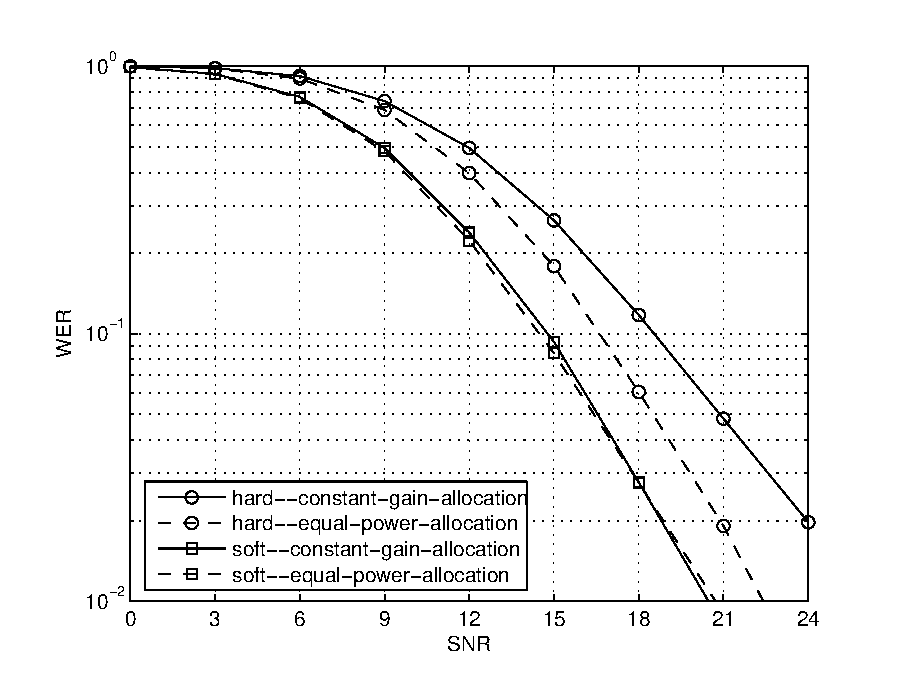
\includegraphics[width=3in]{sp_af_wer_m1_TU.eps} \label{fig:sp_af_wer_m1_TU}} 
	\subfigure[m=2]{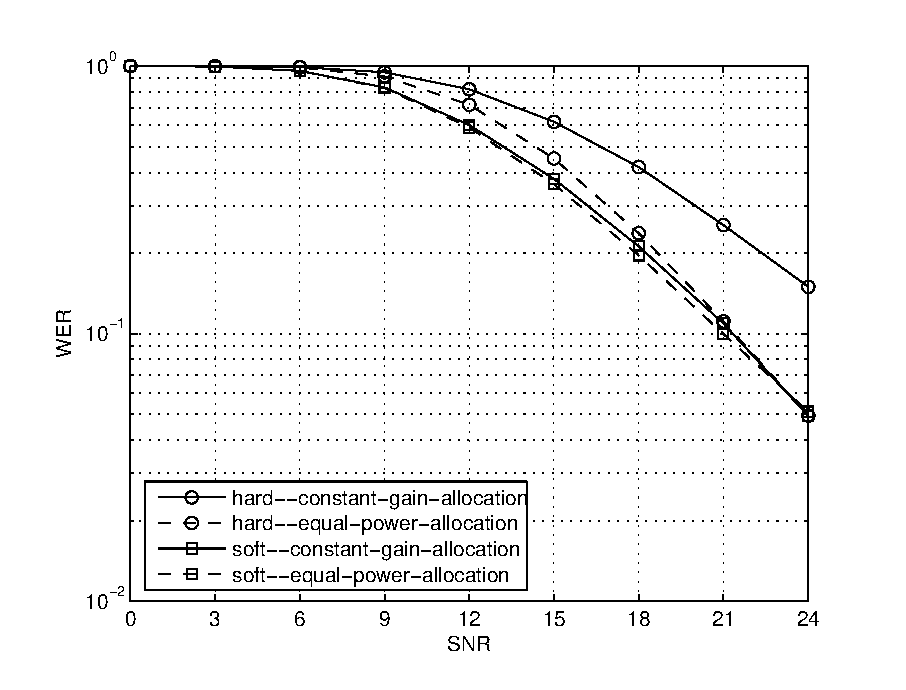
\includegraphics[width=3in]{sp_af_wer_m2_TU.eps} \label{}} \\
}
\centerline{
	\subfigure[m=3]{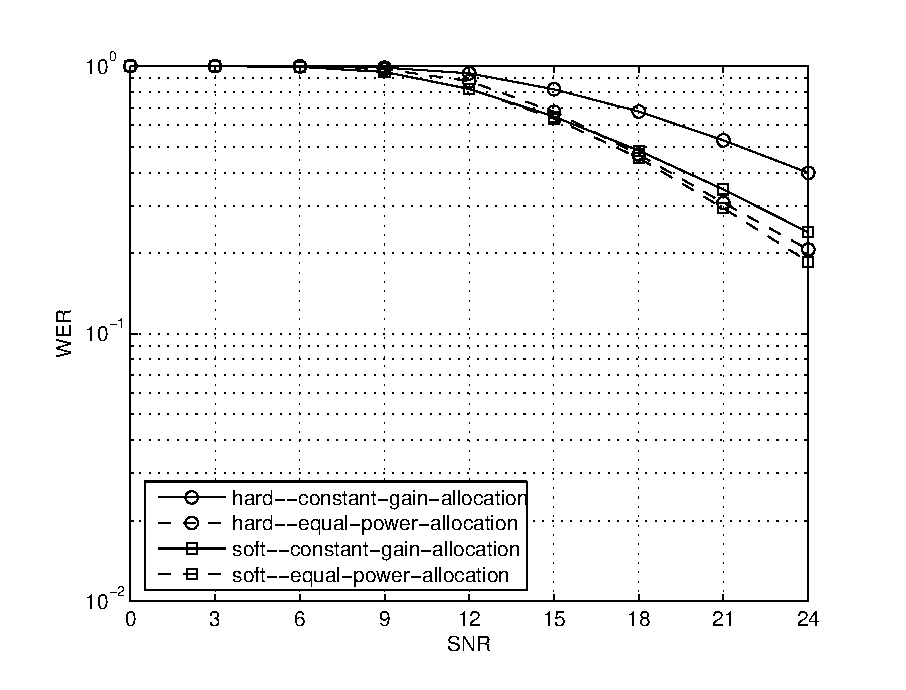
\includegraphics[width=3in]{sp_af_wer_m3_TU.eps} \label{}}
	\subfigure[m=4]{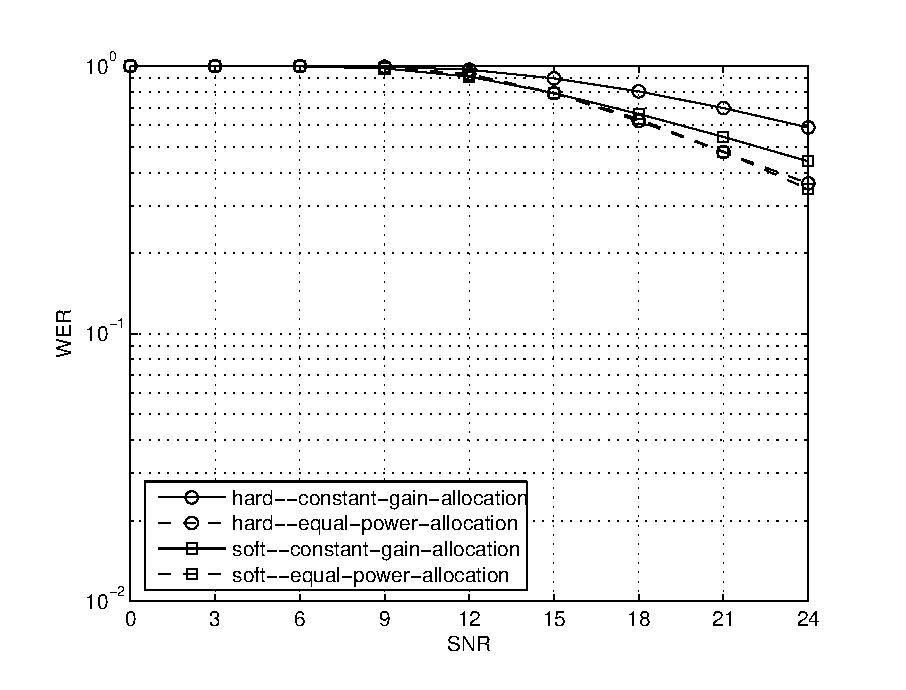
\includegraphics[width=3in]{sp_af_wer_m4_TU.eps} \label{}} \\
}
\caption{WER in a single path relay network with TU channels using AF.  $N = 128, m = 1, 2, 3$, and $4$.}
\label{fig:sp_af_wer_plots_TU}
\end{figure*}

\begin{figure*}
    \psfrag{BER}[Bc][tc][0.8]{BER}
    \psfrag{SNR}[tc][Bc][0.8]{SNR (dB)}
    \psfrag{hard--constant-gain-allocation}[cl][cl][0.5]{hard, constant gain allocation}
    \psfrag{hard--equal-power-allocation}[cl][cl][0.5]{hard, equal power allocation}
    \psfrag{soft--constant-gain-allocation}[cl][cl][0.5]{soft, constant gain allocation}
    \psfrag{soft--equal-power-allocation}[cl][cl][0.5]{soft, equal power allocation}

\centerline{
	\subfigure[m=1]{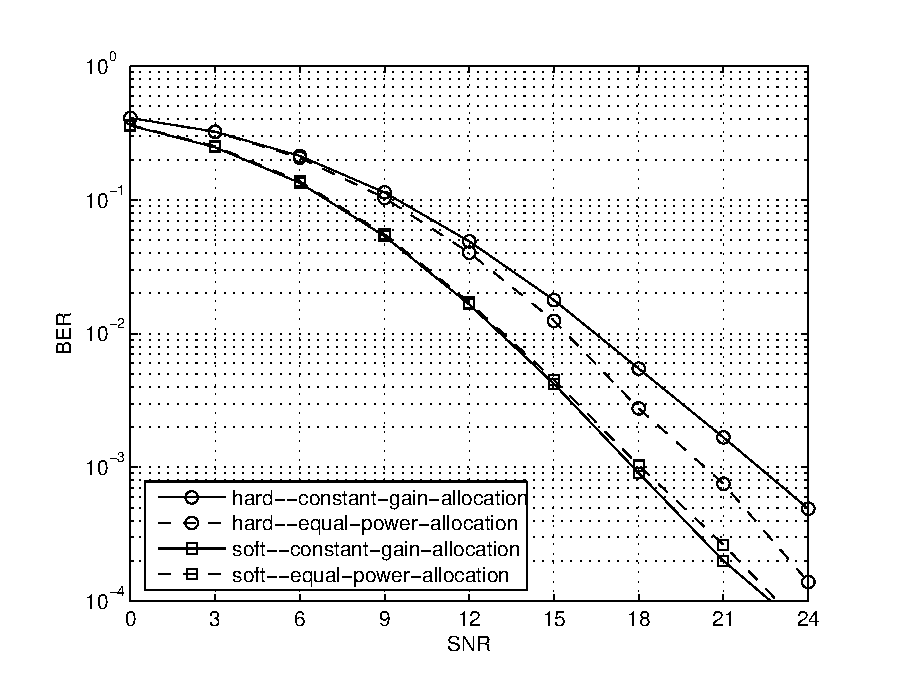
\includegraphics[width=3in]{sp_af_ber_m1_HT.eps} \label{fig:sp_af_ber_m1_HT}} 
	\subfigure[m=2]{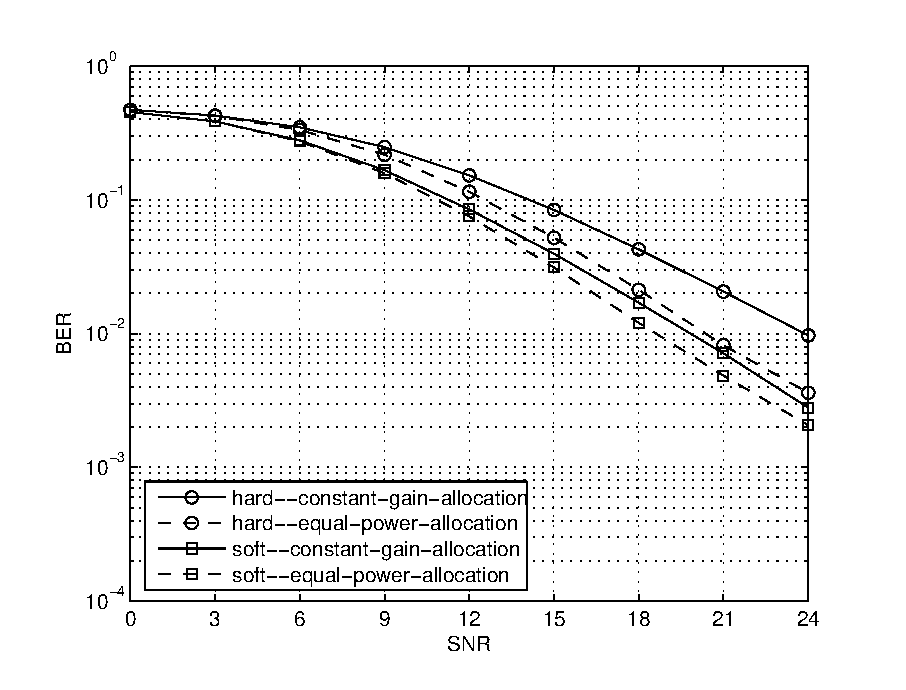
\includegraphics[width=3in]{sp_af_ber_m2_HT.eps} \label{}} \\
}
\centerline{
	\subfigure[m=3]{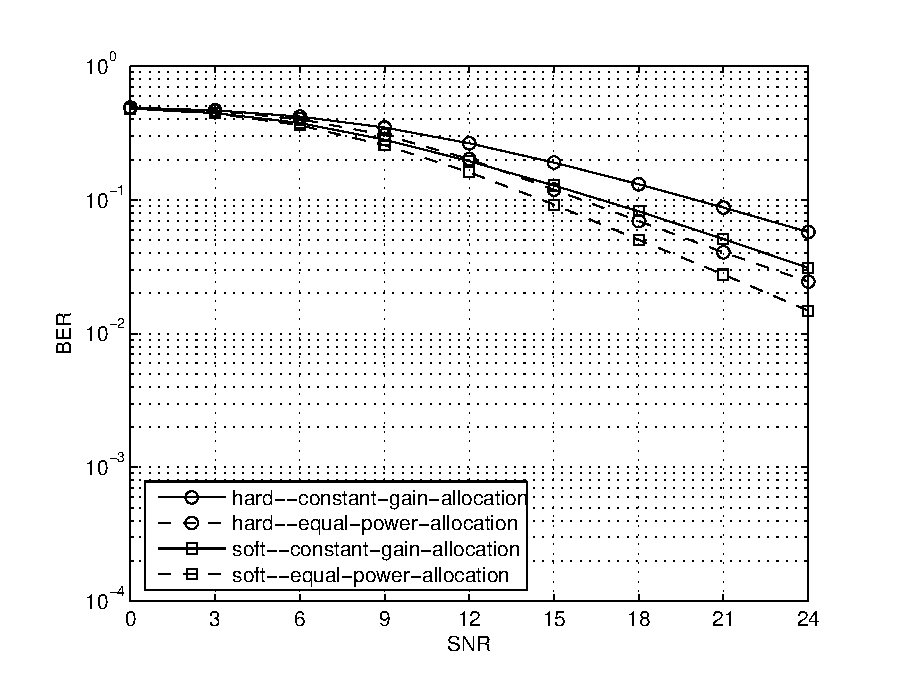
\includegraphics[width=3in]{sp_af_ber_m3_HT.eps} \label{}}
	\subfigure[m=4]{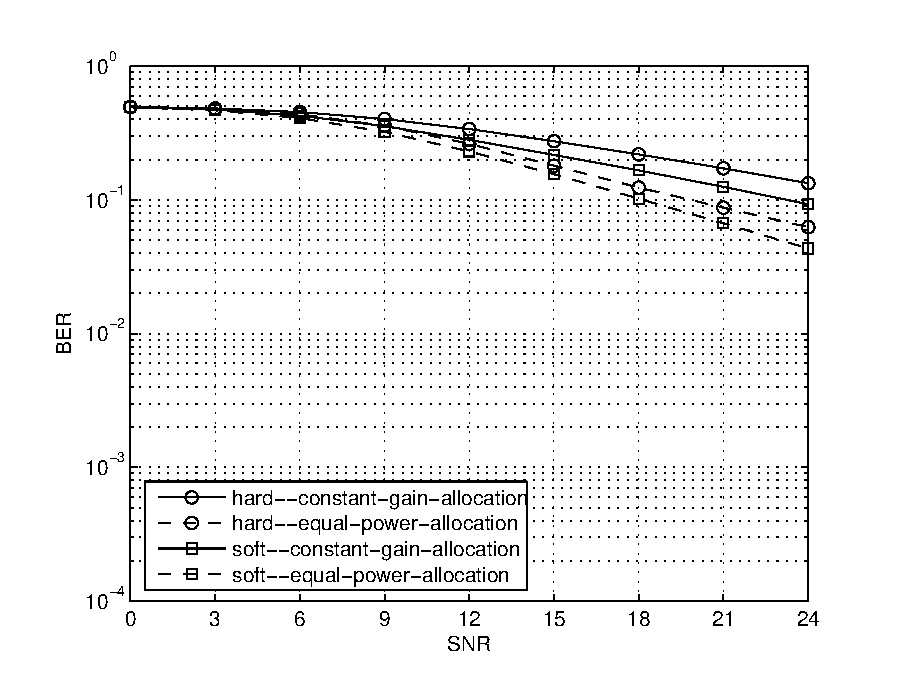
\includegraphics[width=3in]{sp_af_ber_m4_HT.eps} \label{}} \\
}
\caption{BER in a single path relay network with HT channels using AF.  $N = 128, m = 1, 2, 3$, and $4$.}
\label{fig:sp_af_ber_plots_HT}
\end{figure*}

\begin{figure*}
    \psfrag{WER}[Bc][tc][0.8]{WER}
    \psfrag{SNR}[tc][Bc][0.8]{SNR (dB)}
    \psfrag{hard--constant-gain-allocation}[cl][cl][0.5]{hard, constant gain allocation}
    \psfrag{hard--equal-power-allocation}[cl][cl][0.5]{hard, equal power allocation}
    \psfrag{soft--constant-gain-allocation}[cl][cl][0.5]{soft, constant gain allocation}
    \psfrag{soft--equal-power-allocation}[cl][cl][0.5]{soft, equal power allocation}

\centerline{
	\subfigure[m=1]{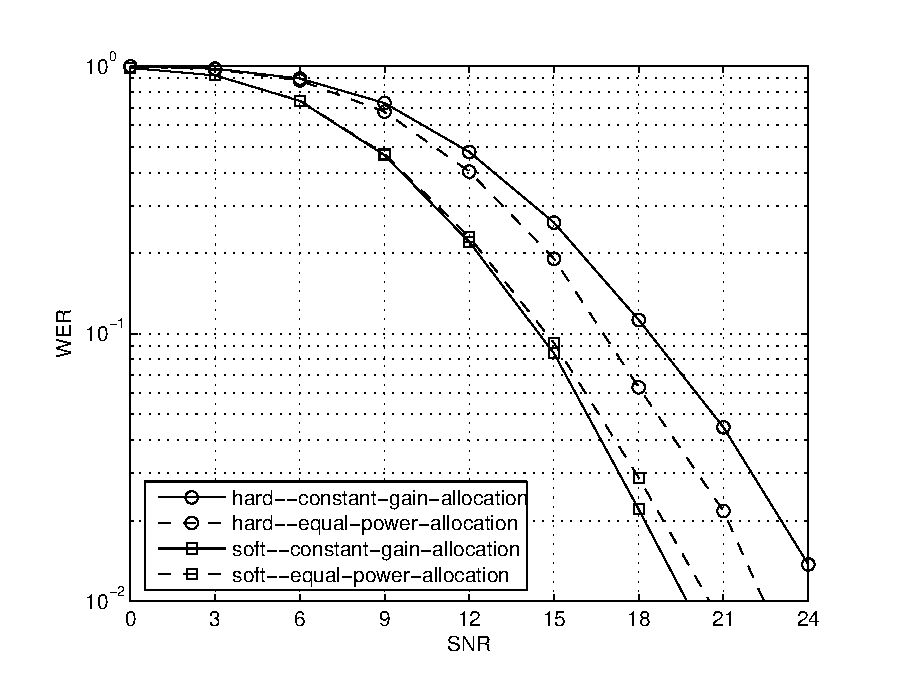
\includegraphics[width=3in]{sp_af_wer_m1_HT.eps} \label{fig:sp_af_wer_m1_HT}} 
	\subfigure[m=2]{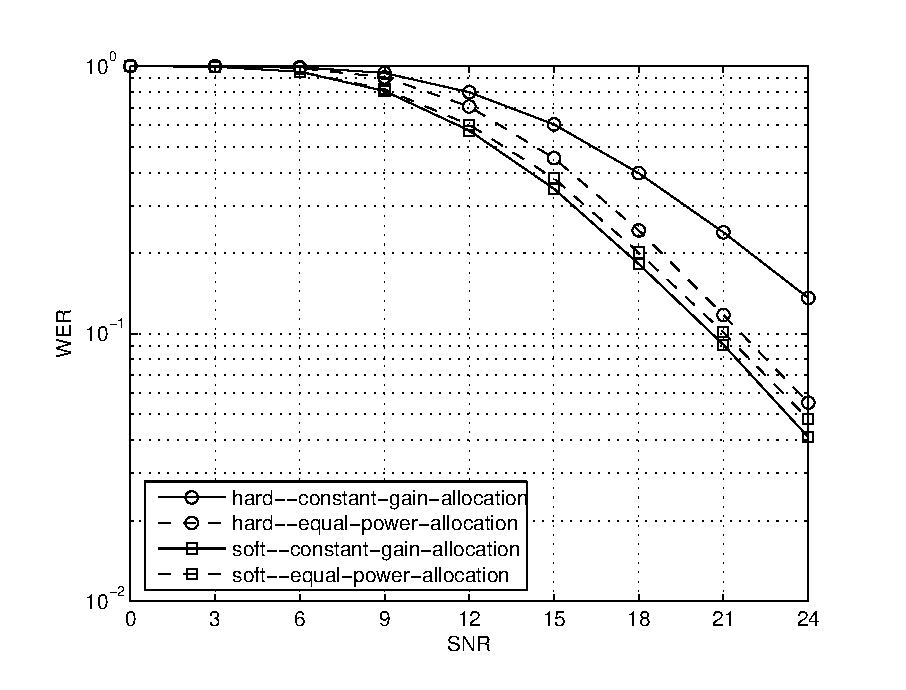
\includegraphics[width=3in]{sp_af_wer_m2_HT.eps} \label{}} \\
}
\centerline{
	\subfigure[m=3]{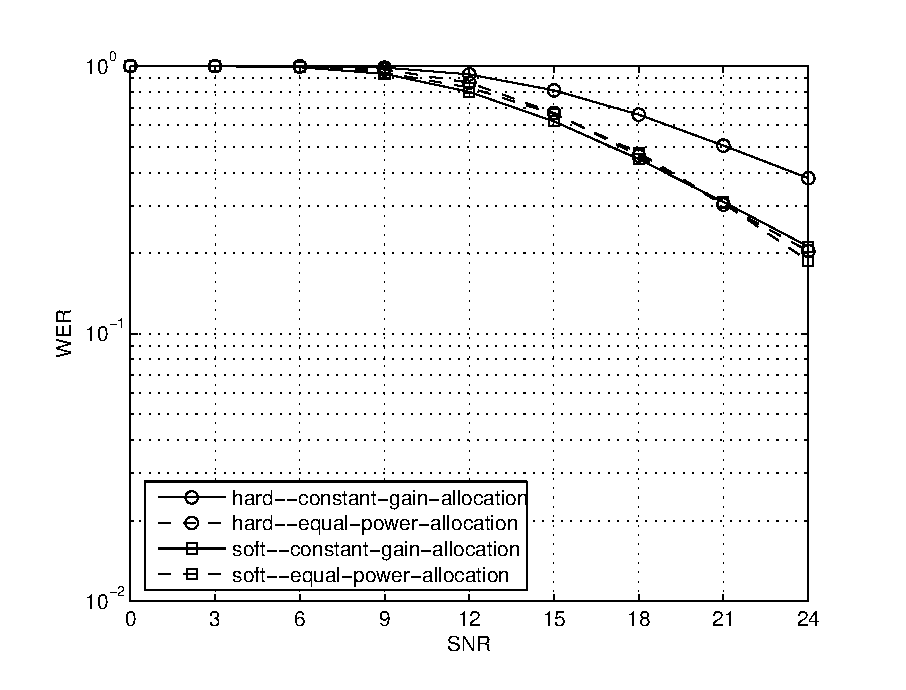
\includegraphics[width=3in]{sp_af_wer_m3_HT.eps} \label{}}
	\subfigure[m=4]{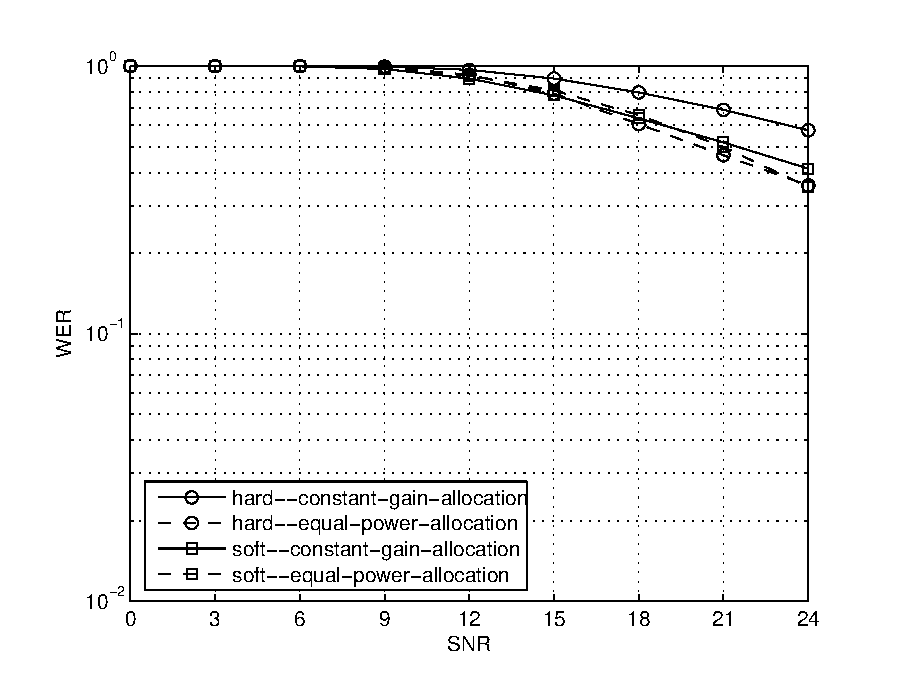
\includegraphics[width=3in]{sp_af_wer_m4_HT.eps} \label{}} \\
}
\caption{WER in a single path relay network with HT channels using AF.  $N = 128, m = 1, 2, 3$, and $4$.}
\label{fig:sp_af_wer_plots_HT}
\end{figure*}

\subsection{Decode-and-Forward}
\label{subsec:sp_bws_df}

The BER versus SNR and WER versus SNR plots for a single path relay network with TU channels using decode-and-forward are shown in Figures \ref{fig:sp_df_ber_plots_TU} and \ref{fig:sp_df_wer_plots_TU}, respectively.  The corresponding plots for HT channels are shown in Figures \ref{fig:sp_df_ber_plots_HT} and \ref{fig:sp_df_wer_plots_HT}, respectively.

As expected, soft decisions in Viterbi decoding give better performance than hard decisions.  In particular, there is up to 5 dB of SNR gain, as shown in the plots.

As we increase the distance between the transmitter and receiver (and thus, add more relays), more noise and channel distortion enter the system.  However, the error rate (BER and WER) performance suffers only slightly as $m$ increases.  TU channels and HT channels give very similar results.

\begin{figure*}
    \psfrag{BER}[Bc][tc][0.8]{BER}
    \psfrag{SNR}[tc][Bc][0.8]{SNR (dB)}
    \psfrag{hard}[cl][cl][0.5]{hard}
    \psfrag{soft}[cl][cl][0.5]{soft}

\centerline{
	\subfigure[m=1]{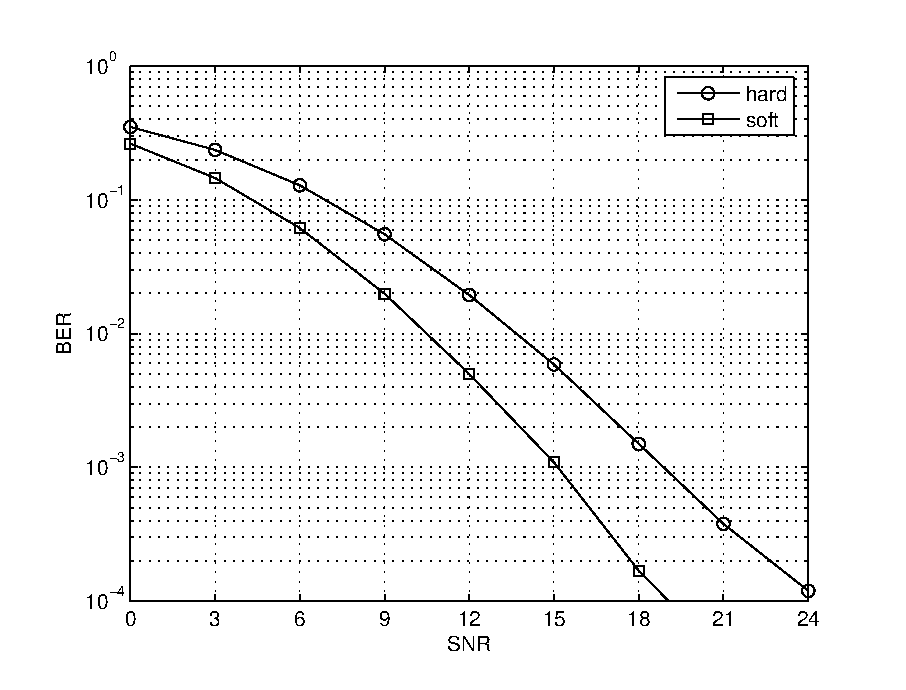
\includegraphics[width=3in]{sp_df_ber_m1_TU.eps} \label{}} 
	\subfigure[m=2]{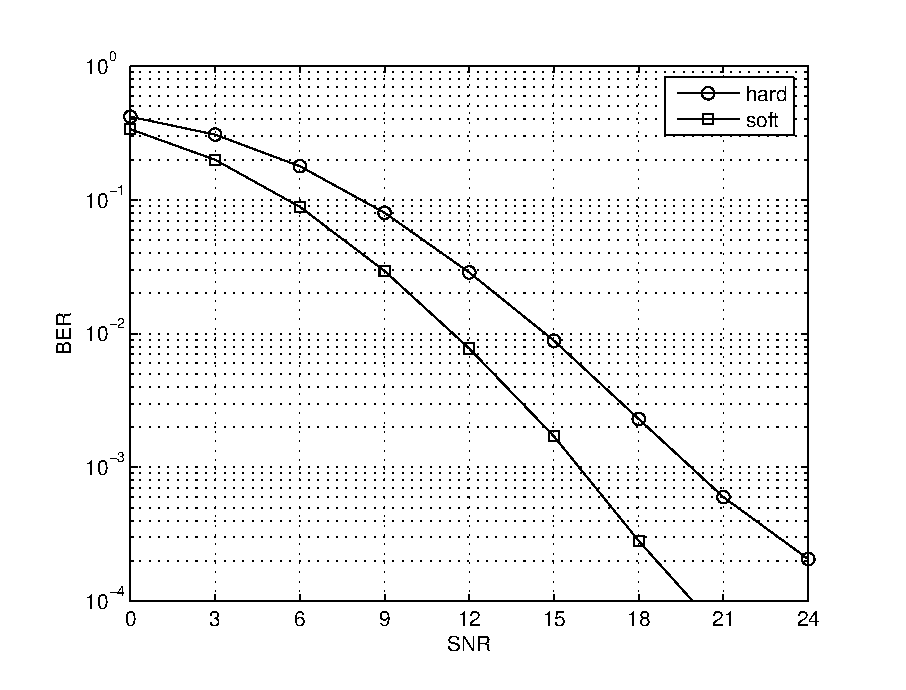
\includegraphics[width=3in]{sp_df_ber_m2_TU.eps} \label{}} \\
}
\centerline{
	\subfigure[m=3]{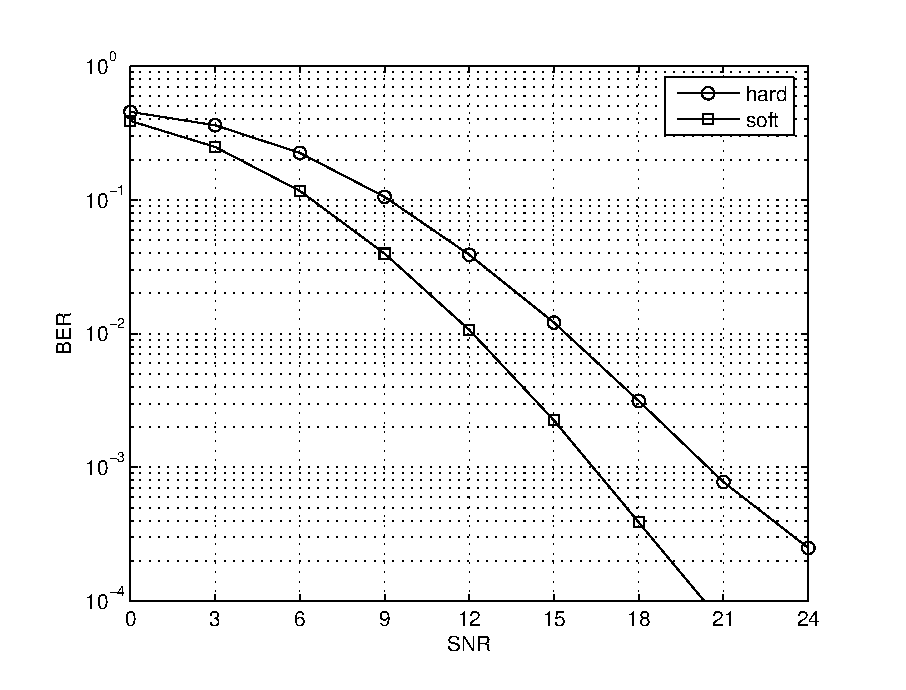
\includegraphics[width=3in]{sp_df_ber_m3_TU.eps} \label{}}
	\subfigure[m=4]{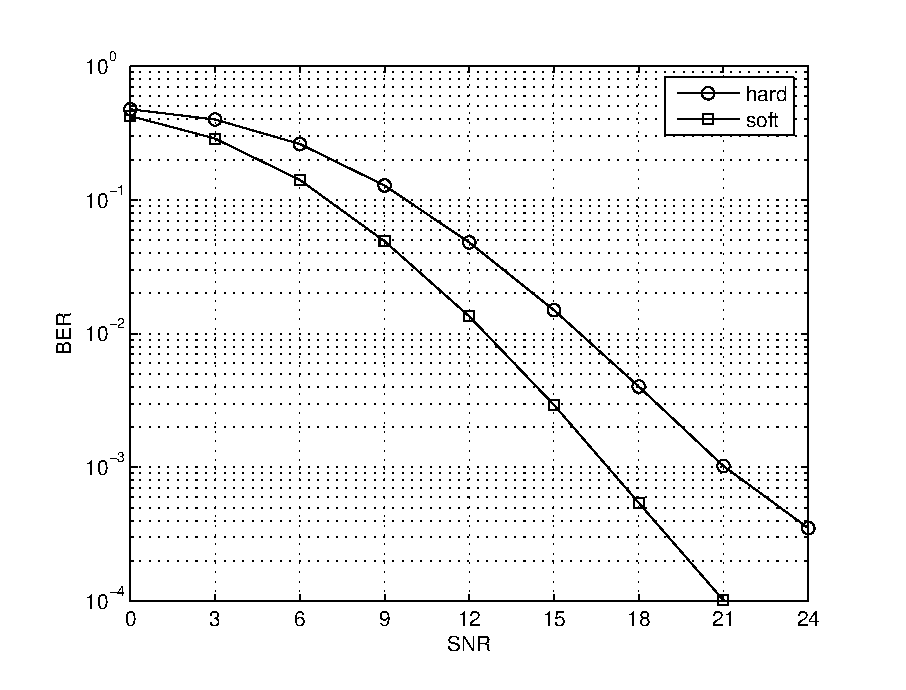
\includegraphics[width=3in]{sp_df_ber_m4_TU.eps} \label{}} \\
}
\caption{BER in a single path relay network with TU channels using DF.  $N = 128, m = 1, 2, 3$, and $4$.}
\label{fig:sp_df_ber_plots_TU}
\end{figure*}

\begin{figure*}
    \psfrag{WER}[Bc][tc][0.8]{WER}
    \psfrag{SNR}[tc][Bc][0.8]{SNR (dB)}
    \psfrag{hard}[cl][cl][0.5]{hard}
    \psfrag{soft}[cl][cl][0.5]{soft}

\centerline{
	\subfigure[m=1]{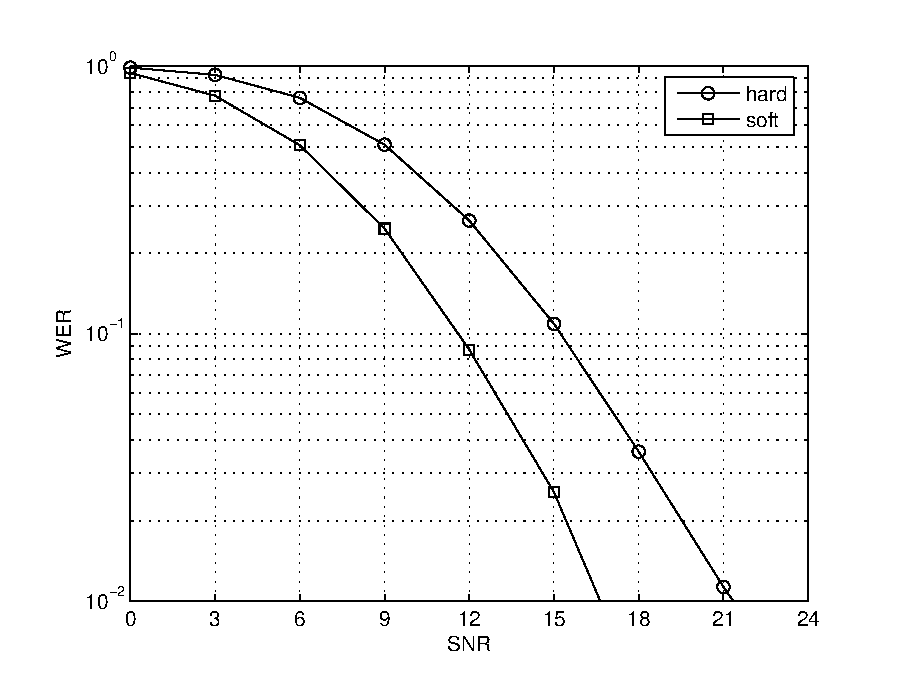
\includegraphics[width=3in]{sp_df_wer_m1_TU.eps} \label{}} 
	\subfigure[m=2]{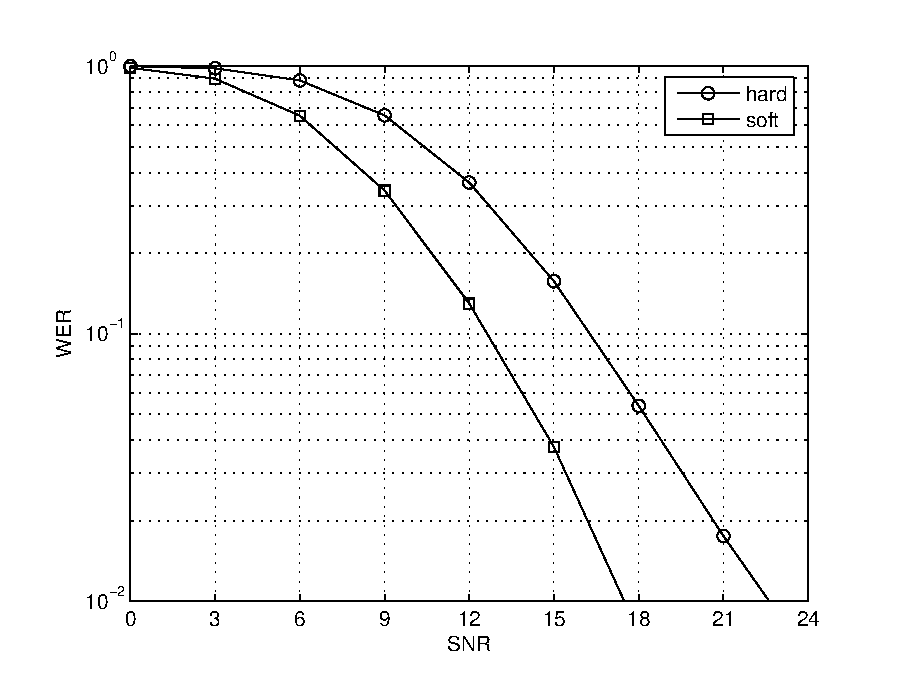
\includegraphics[width=3in]{sp_df_wer_m2_TU.eps} \label{}} \\
}
\centerline{
	\subfigure[m=3]{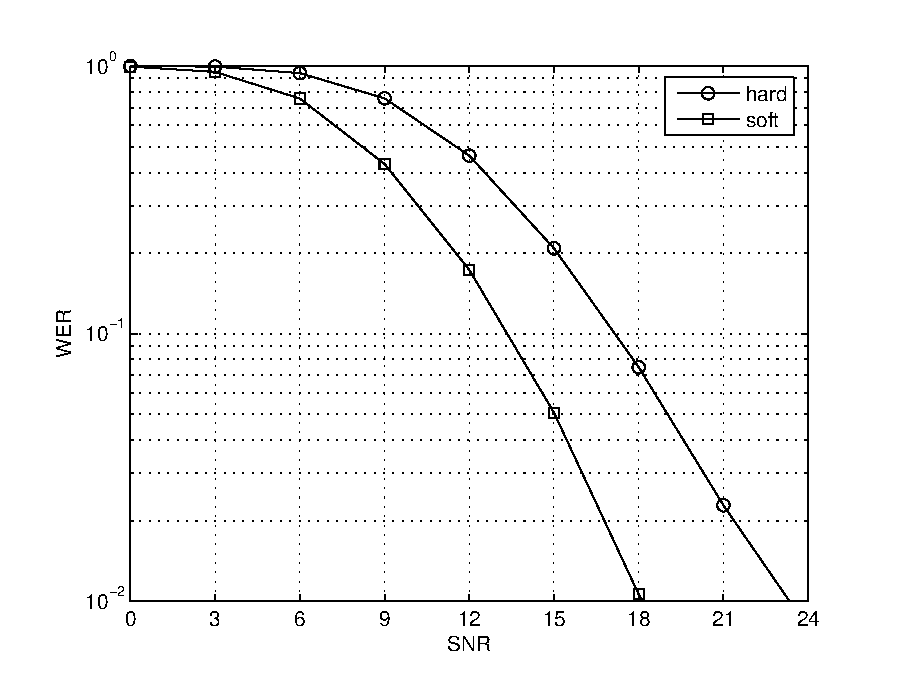
\includegraphics[width=3in]{sp_df_wer_m3_TU.eps} \label{}}
	\subfigure[m=4]{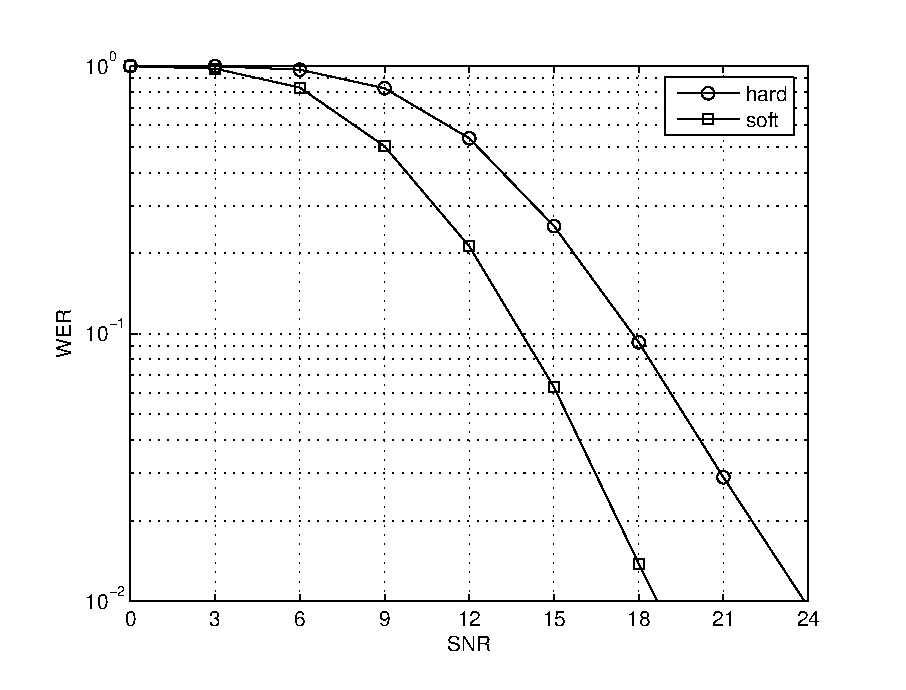
\includegraphics[width=3in]{sp_df_wer_m4_TU.eps} \label{}} \\
}
\caption{WER in a single path relay network with TU channels using DF.  $N = 128, m = 1, 2, 3$, and $4$.}
\label{fig:sp_df_wer_plots_TU}
\end{figure*}

\begin{figure*}
    \psfrag{BER}[Bc][tc][0.8]{BER}
    \psfrag{SNR}[tc][Bc][0.8]{SNR (dB)}
    \psfrag{hard}[cl][cl][0.5]{hard}
    \psfrag{soft}[cl][cl][0.5]{soft}

\centerline{
	\subfigure[m=1]{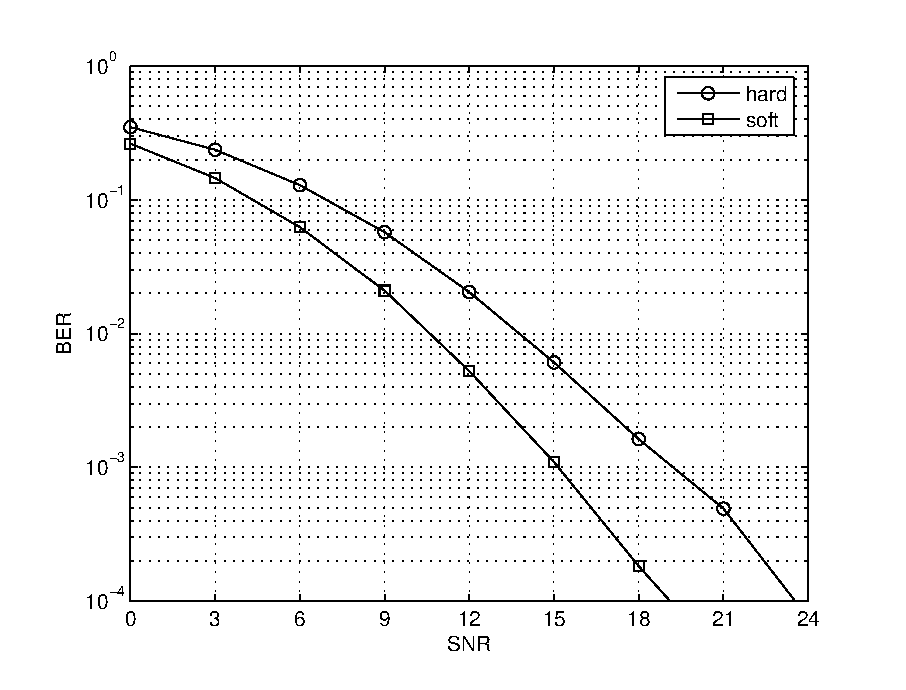
\includegraphics[width=3in]{sp_df_ber_m1_HT.eps} \label{}} 
	\subfigure[m=2]{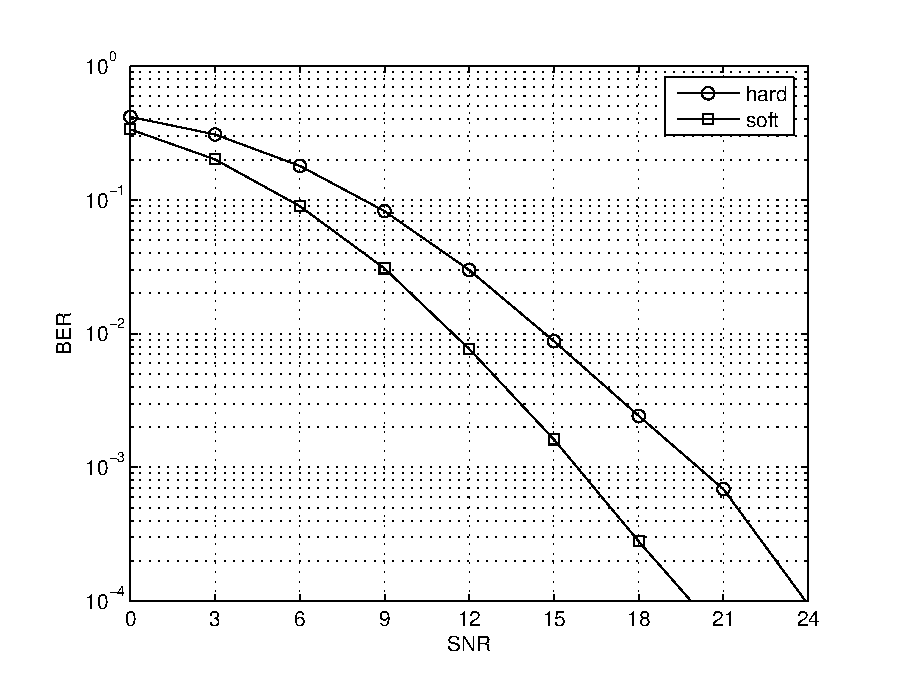
\includegraphics[width=3in]{sp_df_ber_m2_HT.eps} \label{}} \\
}
\centerline{
	\subfigure[m=3]{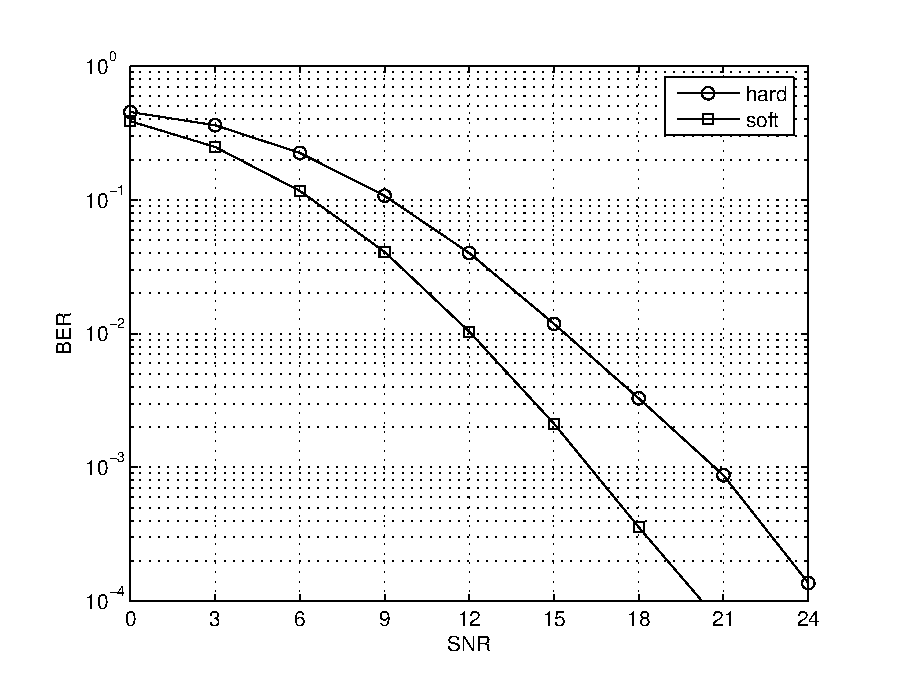
\includegraphics[width=3in]{sp_df_ber_m3_HT.eps} \label{}}
	\subfigure[m=4]{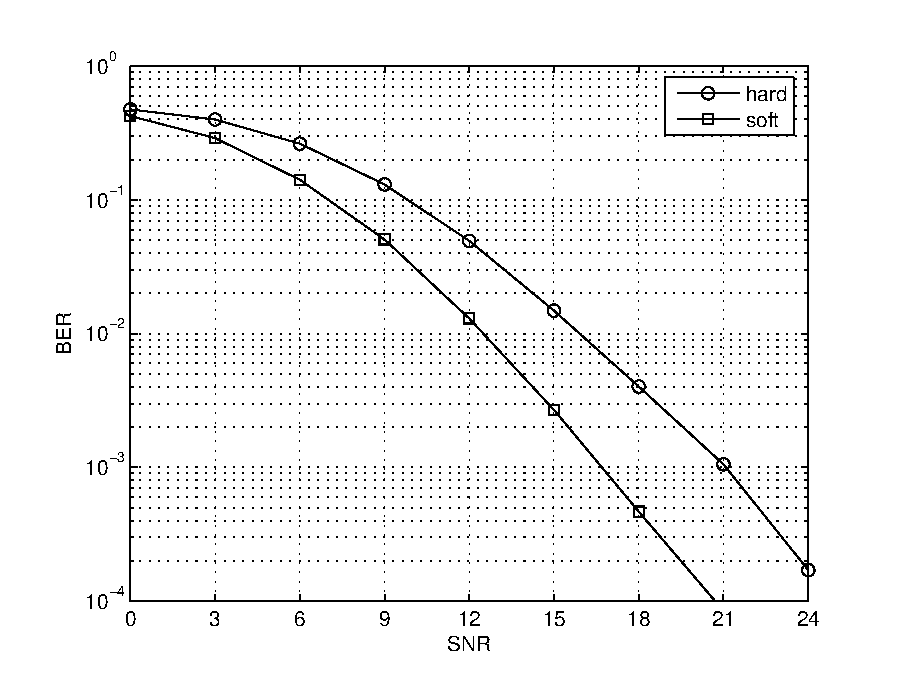
\includegraphics[width=3in]{sp_df_ber_m4_HT.eps} \label{}} \\
}
\caption{BER in a single path relay network with HT channels using DF.  $N = 128, m = 1, 2, 3$, and $4$.}
\label{fig:sp_df_ber_plots_HT}
\end{figure*}

\begin{figure*}
    \psfrag{WER}[Bc][tc][0.8]{WER}
    \psfrag{SNR}[tc][Bc][0.8]{SNR (dB)}
    \psfrag{hard}[cl][cl][0.5]{hard}
    \psfrag{soft}[cl][cl][0.5]{soft}

\centerline{
	\subfigure[m=1]{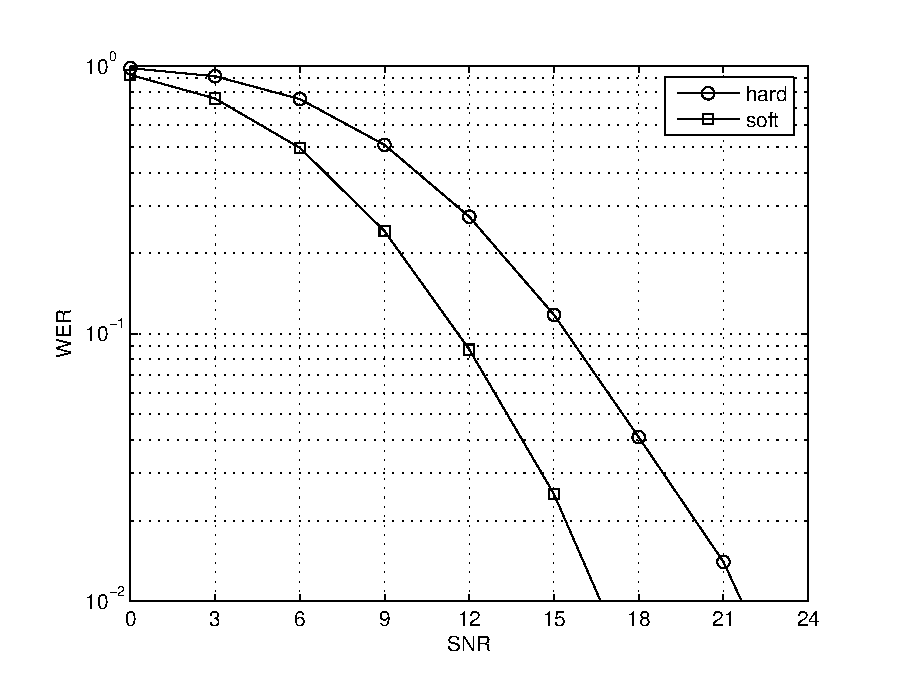
\includegraphics[width=3in]{sp_df_wer_m1_HT.eps} \label{}} 
	\subfigure[m=2]{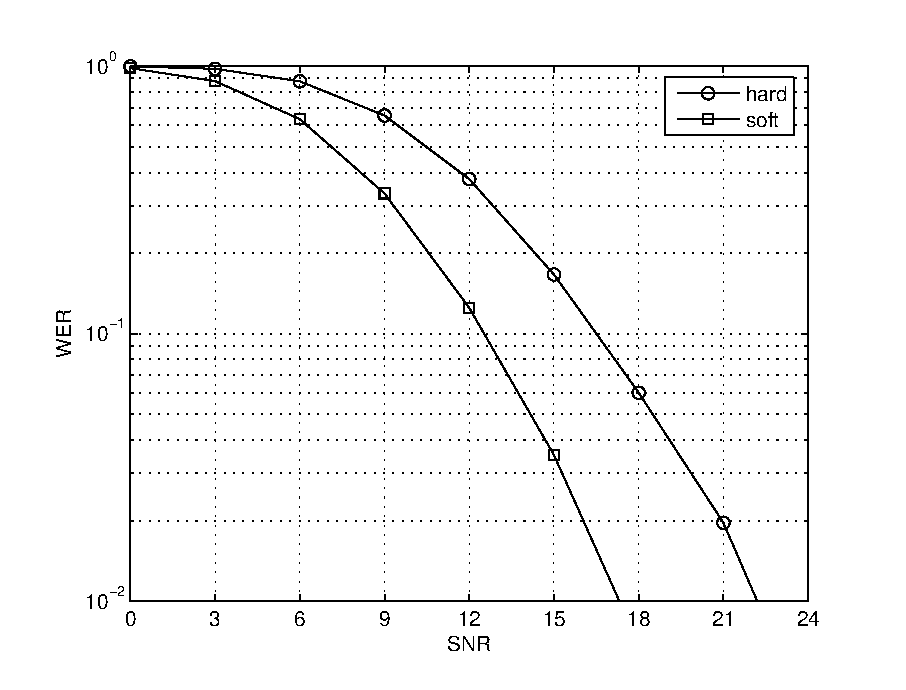
\includegraphics[width=3in]{sp_df_wer_m2_HT.eps} \label{}} \\
}
\centerline{
	\subfigure[m=3]{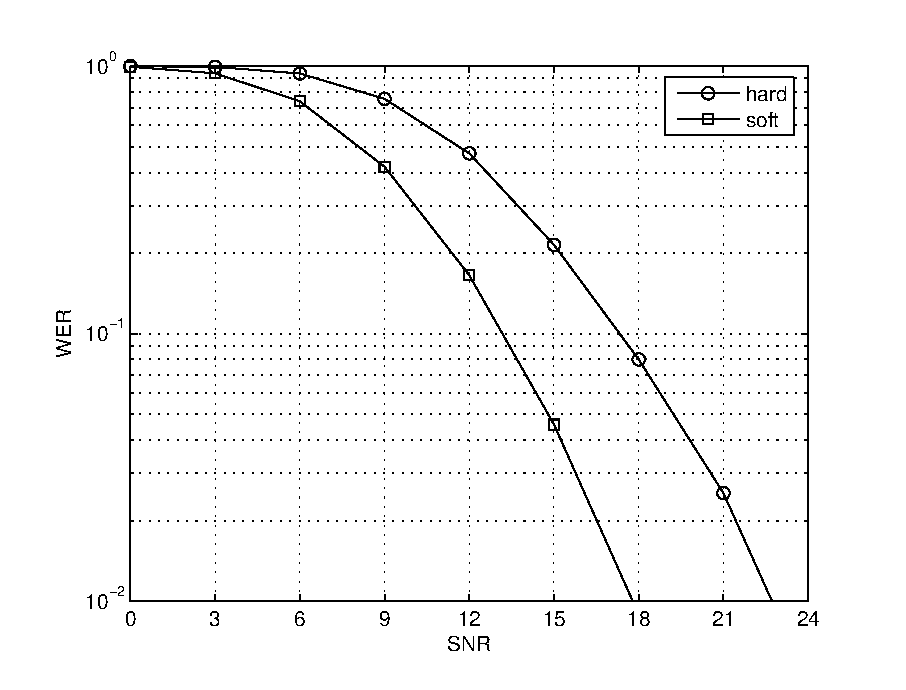
\includegraphics[width=3in]{sp_df_wer_m3_HT.eps} \label{}}
	\subfigure[m=4]{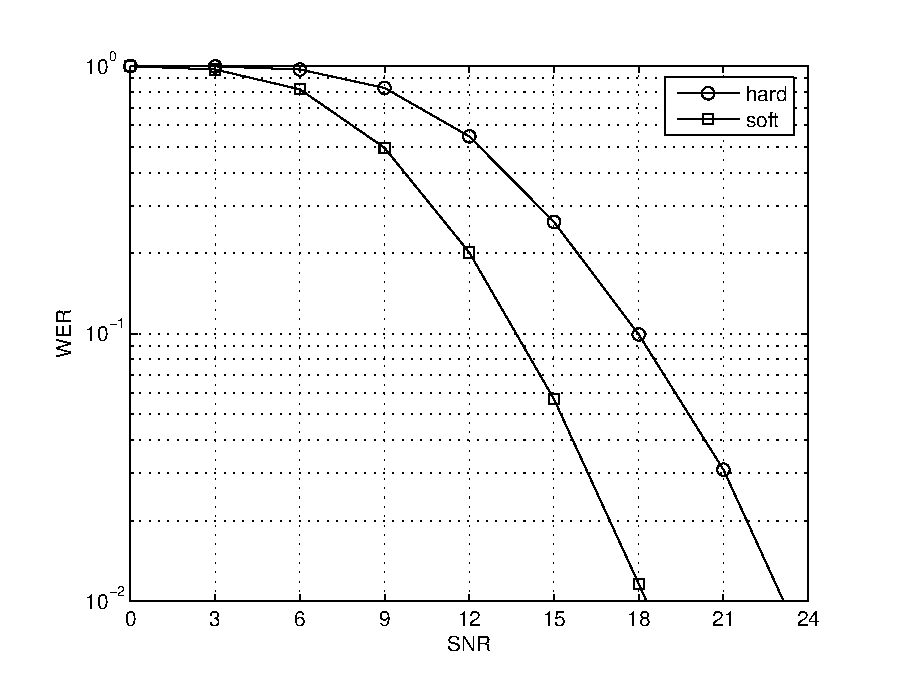
\includegraphics[width=3in]{sp_df_wer_m4_HT.eps} \label{}} \\
}
\caption{WER in a single path relay network with HT channels using DF.  $N = 128, m = 1, 2, 3$, and $4$.}
\label{fig:sp_df_wer_plots_HT}
\end{figure*}

\subsection{Comparison}
\label{subsec:sp_bws_c}

The BER versus SNR and WER versus SNR plots for a single path relay network with TU channels using amplify-and-forward and decode-and-forward are shown in Figures \ref{fig:sp_af_df_ber_plots_TU} and \ref{fig:sp_af_df_wer_plots_TU}, respectively.  The corresponding plots for HT channels are shown in Figures \ref{fig:sp_af_df_ber_plots_HT} and \ref{fig:sp_af_df_wer_plots_HT}, respectively.

As shown in the plots, there are significant error rate (BER and WER) performance gains when using decode-and-forward instead of amplify-and-forward.  The gains are even larger when we increase the distance between the transmitter and receiver (and thus, add more relays).  The amplify-and-forward error rates suffer because more noise and channel distortion enter the system.  The decode-and-forward error rates suffer only slightly because noise and channel distortion are eliminated at each relay.  This results in the large performance gains for $m=4$.

\begin{figure*}
    \psfrag{BER}[Bc][tc][0.8]{BER}
    \psfrag{SNR}[tc][Bc][0.8]{SNR (dB)}
    \psfrag{hard-af-ct----}[cl][cl][0.5]{hard, AF, CT}
    \psfrag{hard-af-eq----}[cl][cl][0.5]{hard, AF, EQ}
    \psfrag{hard-df----}[cl][cl][0.5]{hard, DF}
    \psfrag{soft-af-ct----}[cl][cl][0.5]{soft, AF, CT}
    \psfrag{soft-af-eq----}[cl][cl][0.5]{soft, AF, EQ}
    \psfrag{soft-df----}[cl][cl][0.5]{soft, DF}

\centerline{
	\subfigure[m=1]{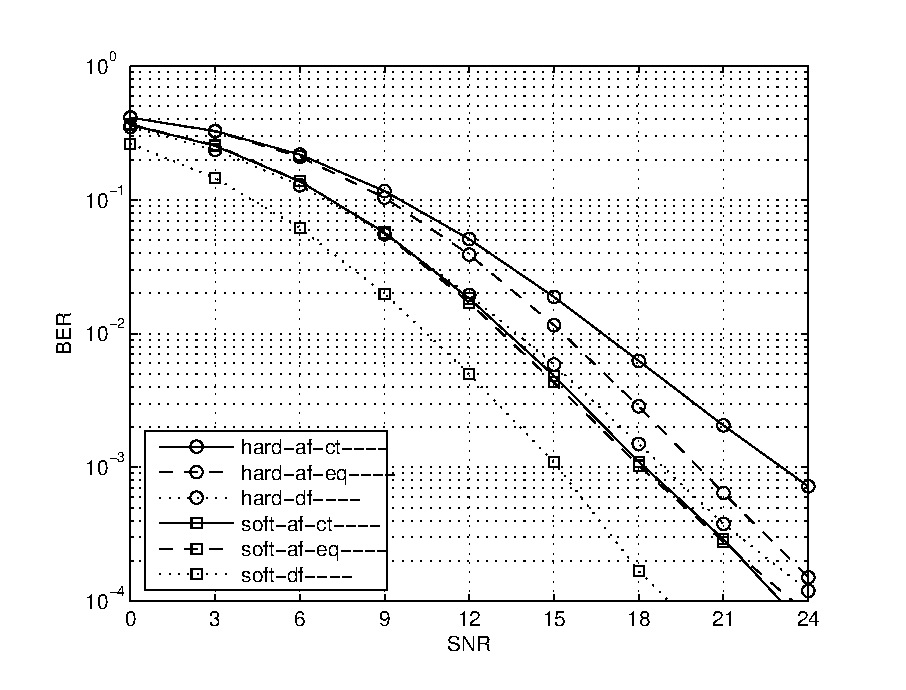
\includegraphics[width=3in]{sp_af_df_ber_m1_TU.eps} \label{}} 
	\subfigure[m=2]{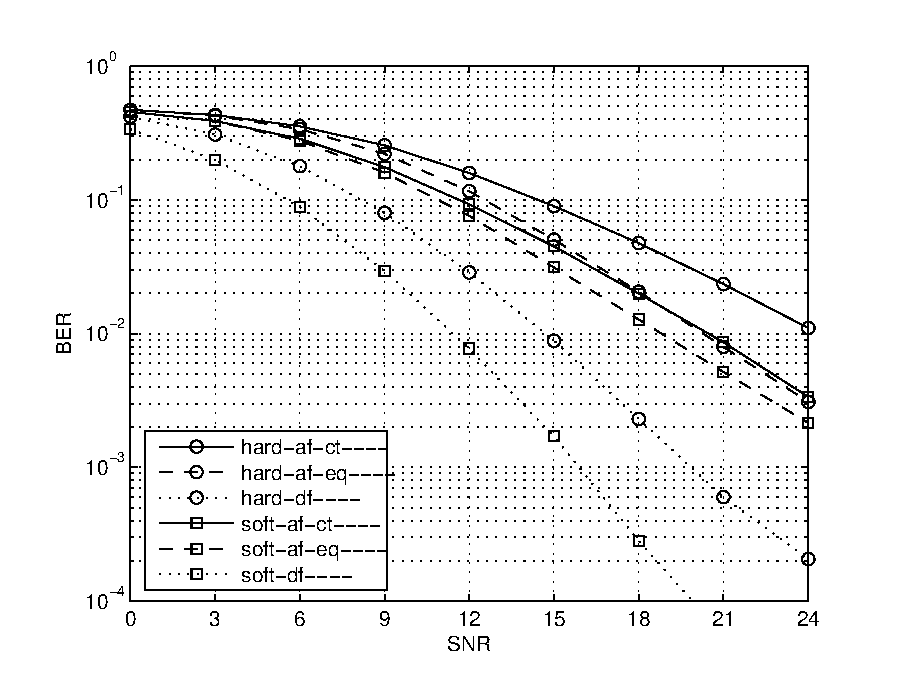
\includegraphics[width=3in]{sp_af_df_ber_m2_TU.eps} \label{}} \\
}
\centerline{
	\subfigure[m=3]{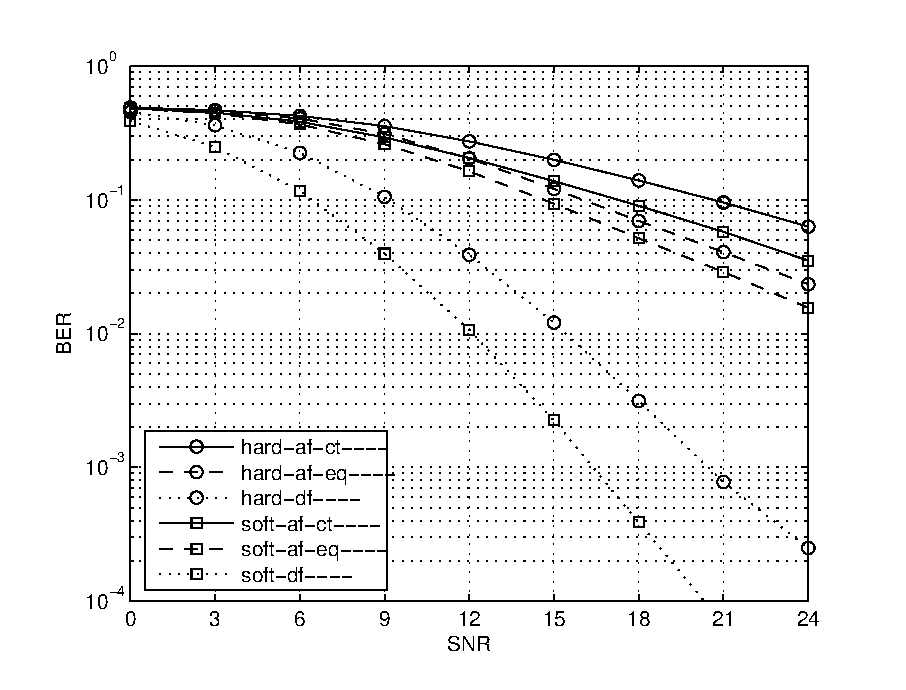
\includegraphics[width=3in]{sp_af_df_ber_m3_TU.eps} \label{}}
	\subfigure[m=4]{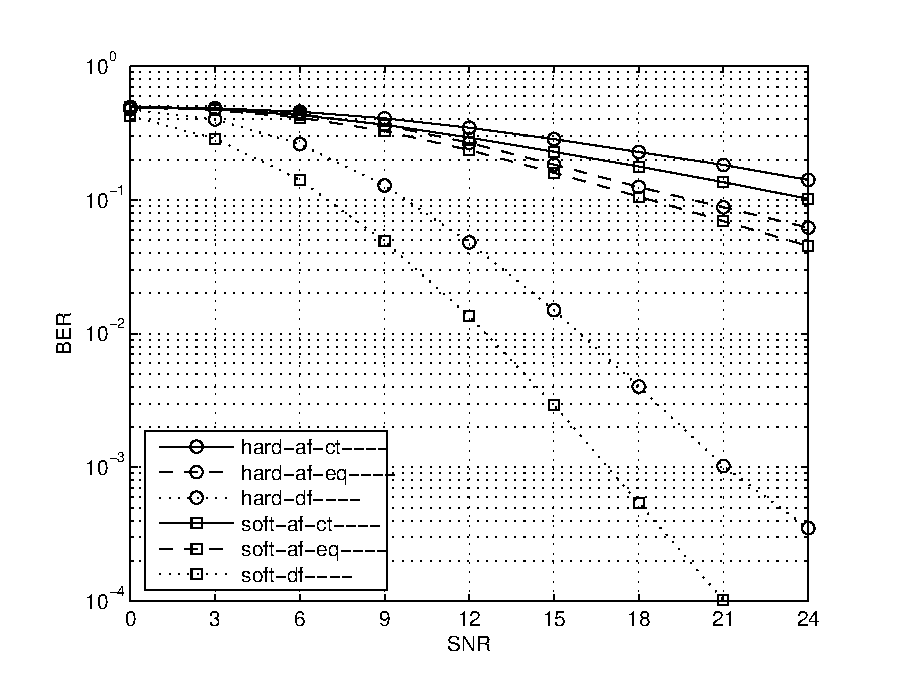
\includegraphics[width=3in]{sp_af_df_ber_m4_TU.eps} \label{}} \\
}
\caption{BER in a single path relay network with TU channels using AF and DF.  $N = 128, m = 1, 2, 3$, and $4$.}
\label{fig:sp_af_df_ber_plots_TU}
\end{figure*}

\begin{figure*}
    \psfrag{WER}[Bc][tc][0.8]{WER}
    \psfrag{SNR}[tc][Bc][0.8]{SNR (dB)}
    \psfrag{hard-af-ct----}[cl][cl][0.5]{hard, AF, CT}
    \psfrag{hard-af-eq----}[cl][cl][0.5]{hard, AF, EQ}
    \psfrag{hard-df----}[cl][cl][0.5]{hard, DF}
    \psfrag{soft-af-ct----}[cl][cl][0.5]{soft, AF, CT}
    \psfrag{soft-af-eq----}[cl][cl][0.5]{soft, AF, EQ}
    \psfrag{soft-df----}[cl][cl][0.5]{soft, DF}

\centerline{
	\subfigure[m=1]{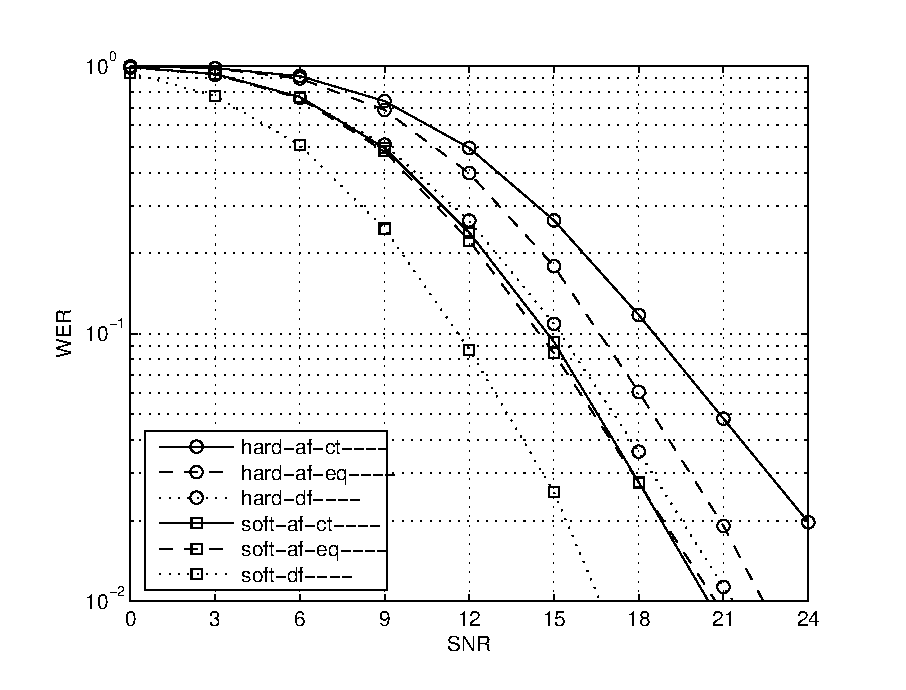
\includegraphics[width=3in]{sp_af_df_wer_m1_TU.eps} \label{}} 
	\subfigure[m=2]{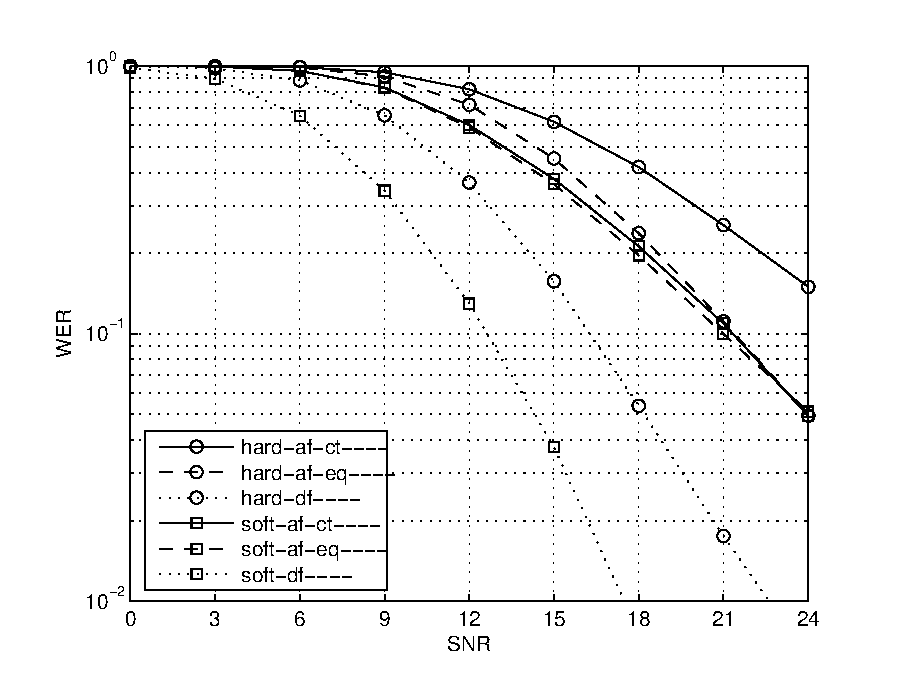
\includegraphics[width=3in]{sp_af_df_wer_m2_TU.eps} \label{}} \\
}
\centerline{
	\subfigure[m=3]{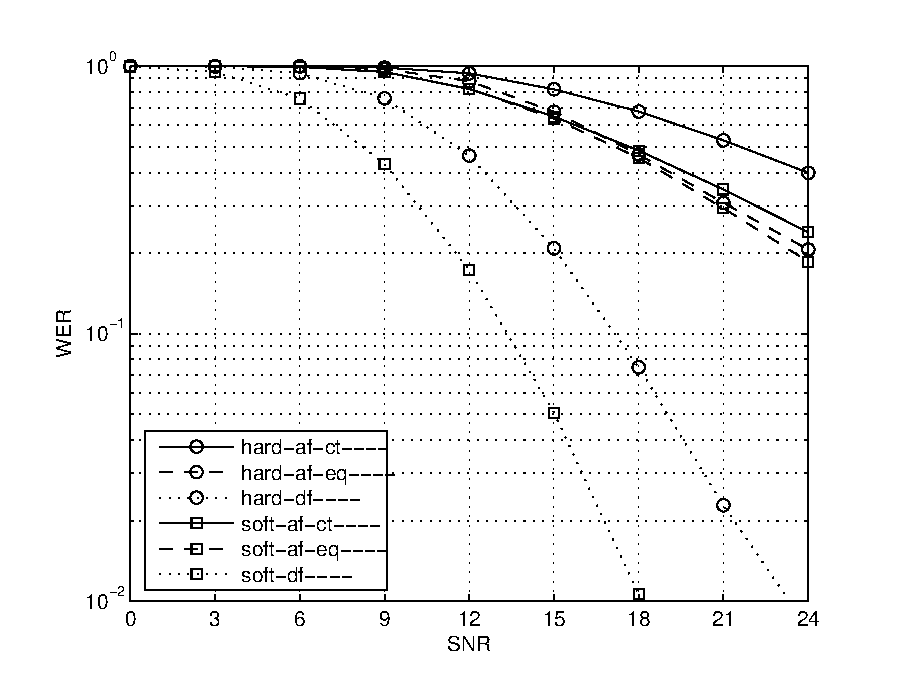
\includegraphics[width=3in]{sp_af_df_wer_m3_TU.eps} \label{}}
	\subfigure[m=4]{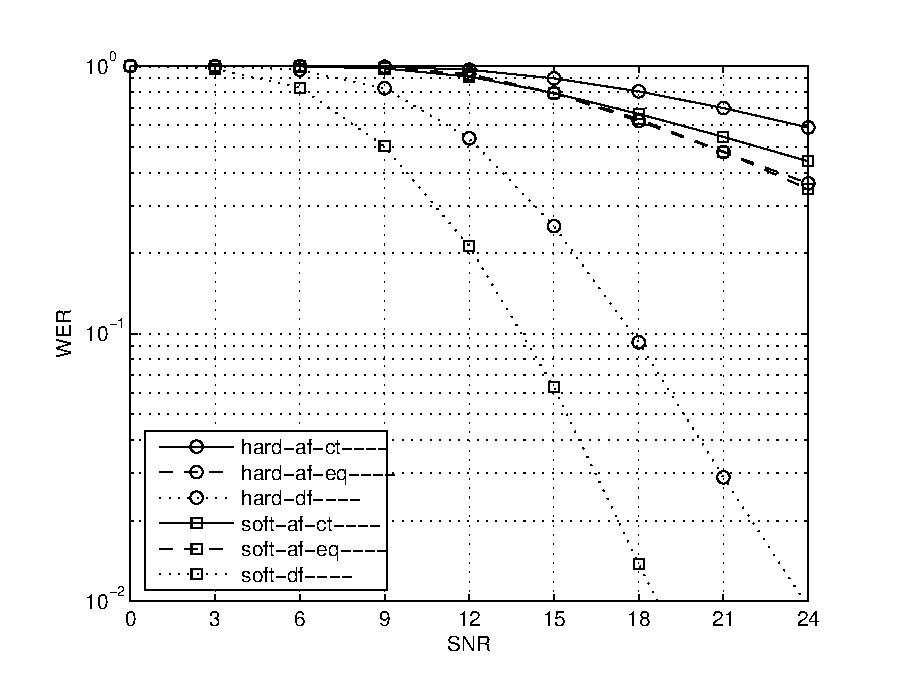
\includegraphics[width=3in]{sp_af_df_wer_m4_TU.eps} \label{}} \\
}
\caption{WER in a single path relay network with TU channels using AF and DF.  $N = 128, m = 1, 2, 3$, and $4$.}
\label{fig:sp_af_df_wer_plots_TU}
\end{figure*}

\begin{figure*}
    \psfrag{BER}[Bc][tc][0.8]{BER}
    \psfrag{SNR}[tc][Bc][0.8]{SNR (dB)}
    \psfrag{hard-af-ct----}[cl][cl][0.5]{hard, AF, CT}
    \psfrag{hard-af-eq----}[cl][cl][0.5]{hard, AF, EQ}
    \psfrag{hard-df----}[cl][cl][0.5]{hard, DF}
    \psfrag{soft-af-ct----}[cl][cl][0.5]{soft, AF, CT}
    \psfrag{soft-af-eq----}[cl][cl][0.5]{soft, AF, EQ}
    \psfrag{soft-df----}[cl][cl][0.5]{soft, DF}

\centerline{
	\subfigure[m=1]{\includegraphics[width=3in]{sp_af_df_ber_m1_HT.eps} \label{}} 
	\subfigure[m=2]{\includegraphics[width=3in]{sp_af_df_ber_m2_HT.eps} \label{}} \\
}
\centerline{
	\subfigure[m=3]{\includegraphics[width=3in]{sp_af_df_ber_m3_HT.eps} \label{}}
	\subfigure[m=4]{\includegraphics[width=3in]{sp_af_df_ber_m4_HT.eps} \label{}} \\
}
\caption{BER in a single path relay network with HT channels using AF and DF.  $N = 128, m = 1, 2, 3$, and $4$.}
\label{fig:sp_af_df_ber_plots_HT}
\end{figure*}

\begin{figure*}
    \psfrag{WER}[Bc][tc][0.8]{WER}
    \psfrag{SNR}[tc][Bc][0.8]{SNR (dB)}
    \psfrag{hard-af-ct----}[cl][cl][0.5]{hard, AF, CT}
    \psfrag{hard-af-eq----}[cl][cl][0.5]{hard, AF, EQ}
    \psfrag{hard-df----}[cl][cl][0.5]{hard, DF}
    \psfrag{soft-af-ct----}[cl][cl][0.5]{soft, AF, CT}
    \psfrag{soft-af-eq----}[cl][cl][0.5]{soft, AF, EQ}
    \psfrag{soft-df----}[cl][cl][0.5]{soft, DF}

\centerline{
	\subfigure[m=1]{\includegraphics[width=3in]{sp_af_df_wer_m1_HT.eps} \label{}} 
	\subfigure[m=2]{\includegraphics[width=3in]{sp_af_df_wer_m2_HT.eps} \label{}} \\
}
\centerline{
	\subfigure[m=3]{\includegraphics[width=3in]{sp_af_df_wer_m3_HT.eps} \label{}}
	\subfigure[m=4]{\includegraphics[width=3in]{sp_af_df_wer_m4_HT.eps} \label{}} \\
}
\caption{WER in a single path relay network with HT channels using AF and DF.  $N = 128, m = 1, 2, 3$, and $4$.}
\label{fig:sp_af_df_wer_plots_HT}
\end{figure*}
